% Options for packages loaded elsewhere
\PassOptionsToPackage{unicode}{hyperref}
\PassOptionsToPackage{hyphens}{url}
%
\documentclass[
]{book}
\usepackage{lmodern}
\usepackage{amssymb,amsmath}
\usepackage{ifxetex,ifluatex}
\ifnum 0\ifxetex 1\fi\ifluatex 1\fi=0 % if pdftex
  \usepackage[T1]{fontenc}
  \usepackage[utf8]{inputenc}
  \usepackage{textcomp} % provide euro and other symbols
\else % if luatex or xetex
  \usepackage{unicode-math}
  \defaultfontfeatures{Scale=MatchLowercase}
  \defaultfontfeatures[\rmfamily]{Ligatures=TeX,Scale=1}
\fi
% Use upquote if available, for straight quotes in verbatim environments
\IfFileExists{upquote.sty}{\usepackage{upquote}}{}
\IfFileExists{microtype.sty}{% use microtype if available
  \usepackage[]{microtype}
  \UseMicrotypeSet[protrusion]{basicmath} % disable protrusion for tt fonts
}{}
\makeatletter
\@ifundefined{KOMAClassName}{% if non-KOMA class
  \IfFileExists{parskip.sty}{%
    \usepackage{parskip}
  }{% else
    \setlength{\parindent}{0pt}
    \setlength{\parskip}{6pt plus 2pt minus 1pt}}
}{% if KOMA class
  \KOMAoptions{parskip=half}}
\makeatother
\usepackage{xcolor}
\IfFileExists{xurl.sty}{\usepackage{xurl}}{} % add URL line breaks if available
\IfFileExists{bookmark.sty}{\usepackage{bookmark}}{\usepackage{hyperref}}
\hypersetup{
  pdftitle={Roberta Spencer Family \& Friends COOKBOOK},
  pdfauthor={The Spencers},
  hidelinks,
  pdfcreator={LaTeX via pandoc}}
\urlstyle{same} % disable monospaced font for URLs
\usepackage{longtable,booktabs}
% Correct order of tables after \paragraph or \subparagraph
\usepackage{etoolbox}
\makeatletter
\patchcmd\longtable{\par}{\if@noskipsec\mbox{}\fi\par}{}{}
\makeatother
% Allow footnotes in longtable head/foot
\IfFileExists{footnotehyper.sty}{\usepackage{footnotehyper}}{\usepackage{footnote}}
\makesavenoteenv{longtable}
\usepackage{graphicx,grffile}
\makeatletter
\def\maxwidth{\ifdim\Gin@nat@width>\linewidth\linewidth\else\Gin@nat@width\fi}
\def\maxheight{\ifdim\Gin@nat@height>\textheight\textheight\else\Gin@nat@height\fi}
\makeatother
% Scale images if necessary, so that they will not overflow the page
% margins by default, and it is still possible to overwrite the defaults
% using explicit options in \includegraphics[width, height, ...]{}
\setkeys{Gin}{width=\maxwidth,height=\maxheight,keepaspectratio}
% Set default figure placement to htbp
\makeatletter
\def\fps@figure{htbp}
\makeatother
\setlength{\emergencystretch}{3em} % prevent overfull lines
\providecommand{\tightlist}{%
  \setlength{\itemsep}{0pt}\setlength{\parskip}{0pt}}
\setcounter{secnumdepth}{5}
\usepackage{wrapfig}

\title{Roberta Spencer Family \& Friends COOKBOOK}
\author{The Spencers}
\date{2021-05-06}

\begin{document}
\maketitle

{
\setcounter{tocdepth}{1}
\tableofcontents
}
\hypertarget{introduction}{%
\chapter{Introduction}\label{introduction}}

This is the Spencer Family \& Friends Cookbook

dedicated to our mother Roberta Belle Spencer who taught us the joy of:

Cooking

Sharing

Eating

Left-overs

Vivamus vehicula leo a justo. Quisque nec augue. Morbi mauris wisi, aliquet vitae, dignissim eget, sollicitudin molestie, ligula. In dictum enim sit amet risus. Curabitur vitae velit eu diam rhoncus hendrerit. Vivamus ut elit. Praesent mattis ipsum quis turpis. Curabitur rhoncus neque eu dui. Etiam vitae magna. Nam ullamcorper. Praesent interdum bibendum magna. Quisque auctor aliquam dolor. Morbi eu lorem et est porttitor fermentum. Nunc egestas arcu at tortor varius viverra. Fusce eu nulla ut nulla interdum consectetuer. Vestibulum gravida.

\begin{wrapfigure}{R}{0.7\textwidth}

\hfill{}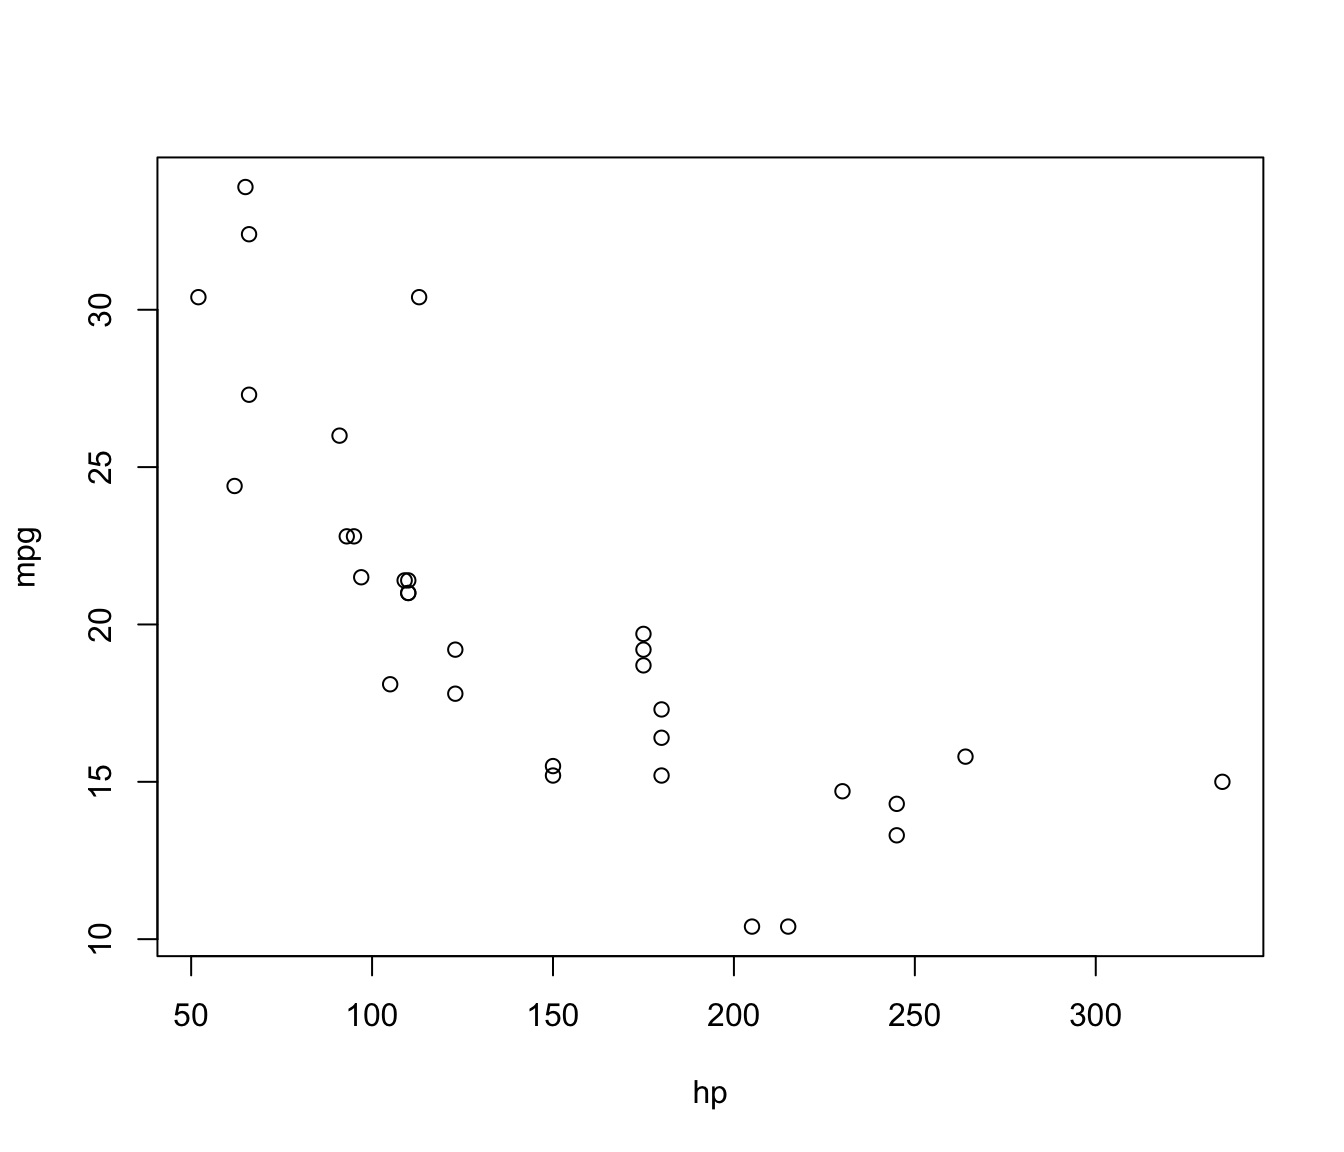
\includegraphics[width=.7\textwidth]{spencerfamilycookbook_files/figure-latex/unnamed-chunk-2-1} 

\caption{My Flowchart}\label{fig:unnamed-chunk-2}
\end{wrapfigure}

Morbi mattis libero sed est. Vivamus vehicula leo a justo. Quisque nec augue. Morbi mauris wisi, aliquet vitae, dignissim eget, sollicitudin molestie, ligula. In dictum enim sit amet risus. Curabitur vitae velit eu diam rhoncus hendrerit. Vivamus ut elit. Praesent mattis ipsum quis turpis. Curabitur rhoncus neque eu dui. Etiam vitae magna. Nam ullamcorper. Praesent interdum bibendum magna. Quisque auctor aliquam dolor. Morbi eu lorem et est porttitor fermentum. Nunc egestas arcu at tortor varius viverra. Fusce eu nulla ut nulla interdum consectetuer. Vestibulum gravida. Morbi mattis libero sed est.

\begin{wrapfigure}{R}{.25\textwidth}  
 \begin{center}
    
\includegraphics[width=.2\textwidth]{"images/500.jpg"}
  \caption{Diamonds} 
\end{center}
\end{wrapfigure}

Morbi mattis libero sed est. Vivamus vehicula leo a justo. Quisque nec augue. Morbi mauris wisi, aliquet vitae, dignissim eget, sollicitudin molestie, ligula. In dictum enim sit amet risus. Curabitur vitae velit eu diam rhoncus hendrerit. Vivamus ut elit. Praesent mattis ipsum quis turpis. Curabitur rhoncus neque eu dui. Etiam vitae magna. Nam ullamcorper. Praesent interdum bibendum magna. Quisque auctor aliquam dolor. Morbi eu lorem et est porttitor fermentum. Nunc egestas arcu at tortor varius viverra. Fusce eu nulla ut nulla interdum consectetuer. Vestibulum gravida. Morbi mattis libero sed est.

Oh yea? Well the same back at you !

\hypertarget{acknowledgements-disclaimers}{%
\chapter*{ACKNOWLEDGEMENTS / DISCLAIMERS}\label{acknowledgements-disclaimers}}


\hypertarget{acknowledgments}{%
\section*{Acknowledgments}\label{acknowledgments}}


Thank you to all that have participated providing recipes for this book. Recipes have been
contributed by family and friends and by many that might not know that we sneaked their recipes,
but good food is worth copying.

\hypertarget{disclaimer}{%
\section*{Disclaimer}\label{disclaimer}}


If there is something you didn't like, you must have made it wrong because we do not make mistakes and
we certainly have great taste. Typing was done by Alvin Spencer who has no ability to spell, count, type or duplicate.
All complaints must be directed to his email Trash Bin within 30 days from the date the recipe was typed.

\hypertarget{cook-and-enjoy}{%
\section*{COOK and ENJOY}\label{cook-and-enjoy}}


\begin{center}\rule{0.5\linewidth}{0.5pt}\end{center}

\hypertarget{notes-notes}{%
\chapter*{NOTES \{\#notes\}}\label{notes-notes}}


\begin{center}\rule{0.5\linewidth}{0.5pt}\end{center}

\hypertarget{notes}{%
\section*{What's the Difference Between Chop, Dice, and Mince?}\label{notes}}


\hypertarget{i-dont-know-but-try-these-comments}{%
\subsection*{I don't know but try these comments}\label{i-dont-know-but-try-these-comments}}


Sometimes the words chop and dice are used interchangeably, but technically the word dice is used for smaller
pieces and the word chop is used for larger pieces.
You seldom see the term large dice, but you will see large chop and small dice rather frequently.
Dice can also refer to cutting vegetable into cubes of a specific size while chop is less precise.
In general, chop is more casual and has more leeway while dice is more specific.
The word mince means a very small dice.

\hypertarget{how-big-is-a-dice-how-small-is-a-mince}{%
\subsection*{How Big is a Dice? How Small is a Mince?}\label{how-big-is-a-dice-how-small-is-a-mince}}


How do you know how big or small something is supposed to be? If the recipe writer feels it matters,
usually they will also include a measurement, like 3/4" dice.
Again, we see the word dice here to indicate that this is a very specific direction.
But if the sizing has some leeway, they will say either large, medium or small chop. Unfortunately,
these sizes aren't standardized so it's hard to give measurements.

\begin{itemize}
\item
  Large chop -- For me, when a recipe says large chop, I usually make it roughly the size of a nickel.
\item
\item
  Medium Chop -- Medium chop is about half the size of a nickel.
\item
\item
  Diced (Small Chop) -- Small chop is about half of medium chop, perhaps a quarter inch to a side.
\item
\item
  Minced -- Mince is very fine, as small as I can get it.
\end{itemize}

\begin{center}\rule{0.5\linewidth}{0.5pt}\end{center}

\hypertarget{appetizers}{%
\chapter{Appetizers and Beverages}\label{appetizers}}

\begin{center}\rule{0.5\linewidth}{0.5pt}\end{center}

\begin{center}\rule{0.5\linewidth}{0.5pt}\end{center}

\hypertarget{artichoke-dip}{%
\section*{ARTICHOKE DIP}\label{artichoke-dip}}


\hypertarget{chef-debbie-wescott}{%
\subsection*{Chef: Debbie Wescott}\label{chef-debbie-wescott}}


\hypertarget{ingredients}{%
\subsection*{Ingredients}\label{ingredients}}


\begin{itemize}
\tightlist
\item
  2 8oz packages of cream cheese - softened
\item
  1/2 cup mayonnaise
\item
  3 to 5 cloves of garlic - or 3 tablespoons of Minced garlic
\item
  14 oz can artichoke hearts drained and chopped - marinated
\item
  10 oz package of frozen spinach - softened
\item
  2 tablespoons of lemon juice
\item
  1/2 cup grated parmesan cheese
\item
  1 cup of mozzoretta cheese - grated
\end{itemize}

\hypertarget{directions}{%
\subsection*{Directions}\label{directions}}


Cream the cream cheese, mayonnaise and garlic together and set aside.
Mix remaining ingredients down the list to Parmesan cheese.
Combine parts 1 and 2 and spread into a baking dish.
Bake at 375 deg for 20 minutes then layer on Mozzoretta cheese,
Bake 5 more minutes until light golden brown.
Serve with fresh veggies or crackers.
YUM!

\begin{center}\rule{0.5\linewidth}{0.5pt}\end{center}

\hypertarget{cowboy-caviar}{%
\section*{COWBOY CAVIAR}\label{cowboy-caviar}}


\hypertarget{chef-patricia-blair}{%
\subsection*{Chef: Patricia Blair}\label{chef-patricia-blair}}


\hypertarget{ingredients-1}{%
\subsection*{Ingredients}\label{ingredients-1}}


\begin{itemize}
\tightlist
\item
  15oz can black eyed peas - drained
\item
  15oz can \href{https://en.wikipedia.org/wiki/Shoepeg_corn}{shoepeg corn} - drained
\item
  2/3 cup cilantro - chopped
\item
  2/3 cup green onion - chopped
\item
  1/4 cup olive oil dressing
\item
  1/4 cup red wine vinegar
\item
  2 cloves garlic - minced
\item
  3/4 teaspoon salt
\item
  1/8 teaspoon pepper
\item
  1/2 teaspoon cumin
\item
  2 large tomatoes - diced
\item
  2 avacados - diced
\end{itemize}

\hypertarget{directions-1}{%
\subsection*{Directions}\label{directions-1}}


Except the tomatoes and avacados marinate all other ingredients together for 6+ hours.
Add diced tomatoes and avacados 30 minutes before serving.

\begin{center}\rule{0.5\linewidth}{0.5pt}\end{center}

\hypertarget{cream-of-coconut-fruit-dip}{%
\section*{CREAM OF COCONUT FRUIT DIP}\label{cream-of-coconut-fruit-dip}}


\hypertarget{chef-jennifer-gustin}{%
\subsection*{Chef: Jennifer Gustin}\label{chef-jennifer-gustin}}


\hypertarget{ingredients-2}{%
\subsection*{Ingredients}\label{ingredients-2}}


\begin{itemize}
\tightlist
\item
  1 package instant vanilla pudding (4.6 oz)
\item
  1 container cream of coconut (found in alcohol mix section)
\item
  16 oz whipped cream (Cool Whip)
\end{itemize}

\hypertarget{directions-2}{%
\subsection*{Directions}\label{directions-2}}


Combine all three ingredients together and chill for one hour so pudding dissolves completely.
Serve with fruit. Great with sliced apple.

\begin{center}\rule{0.5\linewidth}{0.5pt}\end{center}

\hypertarget{cucumber-sandwiches}{%
\section*{CUCUMBER SANDWICHES}\label{cucumber-sandwiches}}


\hypertarget{chef-patricia-blair-1}{%
\subsection*{Chef: Patricia Blair}\label{chef-patricia-blair-1}}


\hypertarget{ingredients-3}{%
\subsection*{Ingredients}\label{ingredients-3}}


\begin{itemize}
\tightlist
\item
  8 oz cream cheese
\item
  2 tablespoons mayonnaise
\item
  2 green onions - diced
\item
  1/2 teaspoon \href{https://www.mccormick.com/gourmet/recipes/other/bon-appetit-seasoning-replacement}{Bon Appettit} seasoning
\item
  1/2 teaspoon dill weed
\item
  1/2 teaspoon garlic salt
\item
  cucumbers - peeled and sliced
\item
  tomatoes - sliced
\item
  bread - crust removed
\end{itemize}

\hypertarget{directions-3}{%
\subsection*{Directions}\label{directions-3}}


Combine together: cream cheese, mayonnaise, green onions, Bon Appettit, dill weed, and garlic salt.
Spread mixture on bread and layer with sliced cucumber and tomato. Cover and refrigerate until ready to use.

\begin{center}\rule{0.5\linewidth}{0.5pt}\end{center}

\hypertarget{dads-sunday-evening-popcorn}{%
\section*{DAD'S SUNDAY EVENING POPCORN}\label{dads-sunday-evening-popcorn}}


\hypertarget{chef-alvin-spencer}{%
\subsection*{Chef: Alvin Spencer}\label{chef-alvin-spencer}}


\hypertarget{ingredients-4}{%
\subsection*{Ingredients}\label{ingredients-4}}


\begin{itemize}
\tightlist
\item
  1/2 cup of popcorn - uncooked
\item
  1 to 3 teaspoons of olive oil
\item
  1/4 cup of butter or margerine
\item
  1/4 teaspoon of popcorn salt
\end{itemize}

\hypertarget{directions-4}{%
\subsection*{Directions}\label{directions-4}}


Best cooked in a \href{https://www.whirleypopshop.com/}{Whirley-pop} popcorn popper. This requires only 1 teaspoon of oil.\\
Cook over medium high heat until kernels stop popping or until smoke fills the kitchen.
Place in a large bowel and sprinkle melted butter lightly over popcorn while stirring. Olive oil can be substituted for margarine.
Sprinkle salt over popcorn and stir. Eat while warm and while watching a good movie with the family gathered around you.

\begin{center}\rule{0.5\linewidth}{0.5pt}\end{center}

\hypertarget{five-layer-avocado-dip}{%
\section*{FIVE LAYER AVOCADO DIP}\label{five-layer-avocado-dip}}


\hypertarget{chef-patricia-blair-2}{%
\subsection*{Chef: Patricia Blair}\label{chef-patricia-blair-2}}


\hypertarget{ingredients-5}{%
\subsection*{Ingredients}\label{ingredients-5}}


\begin{itemize}
\tightlist
\item
  1 can refried beans
\item
  1 can chip bean dip
\item
  2 large avocados - mashed
\item
  1 small can green chilies - diced
\item
  1/2 pint sour cream
\item
  1/4 jar favorite salsa
\item
  garlic / onion salt and pepper
\item
  1/2 cup green onions - chopped
\item
  1 can sliced black olives
\item
  1 lb. favorite shredded cheese
\end{itemize}

\hypertarget{directions-5}{%
\subsection*{Directions}\label{directions-5}}


Layer in 9x13 pan.
-- First Layer: 1 can refried beans and 1 can chip bean dip.
-- Second Layer (Mix together) avocados, green chilies, sour cream, salsa, seasonings.
-- Third Layer: Green onions,
-- Fourth Layer: sliced olives.
-- Fifth Layer: cheese.

Serve with chips

\begin{center}\rule{0.5\linewidth}{0.5pt}\end{center}

\hypertarget{hot-buttered-rum-drink}{%
\section*{HOT BUTTERED `RUM' DRINK}\label{hot-buttered-rum-drink}}


\hypertarget{chef-jennifer-gustin-1}{%
\subsection*{Chef: Jennifer Gustin}\label{chef-jennifer-gustin-1}}


\hypertarget{ingredients-6}{%
\subsection*{Ingredients}\label{ingredients-6}}


\begin{itemize}
\tightlist
\item
  1 1/2 cups brown sugar
\item
  1 3/4 cups powdered sugar
\item
  2 pints vanilla ice-cream
\item
  1/2 teaspoon nutmeg
\item
  1 teaspoon cinnamon
\end{itemize}

\hypertarget{directions-6}{%
\subsection*{Directions}\label{directions-6}}


Soften ice-cream 30 minutes in refrigerator. Mix dry ingredients together.
Cream together dry ingredients with softened ice-cream.
Store in freezer. To serve, use 1 1/2 tsp of batter to a cup of hot water or milk. Add more to taste.

\begin{center}\rule{0.5\linewidth}{0.5pt}\end{center}

\hypertarget{hot-chocolate-mix}{%
\section*{HOT CHOCOLATE MIX}\label{hot-chocolate-mix}}


\hypertarget{chef-roberta-spencer}{%
\subsection*{Chef: Roberta Spencer}\label{chef-roberta-spencer}}


\hypertarget{ingredients-7}{%
\subsection*{Ingredients}\label{ingredients-7}}


\begin{itemize}
\tightlist
\item
  1 25.6 oz package of instant nonfat dry milk (10 2/3 cups)
\item
  1 6 oz jar powdered non-dairy creamer
\item
  2 cups powdered sugar
\item
  1 16 oz can instant chocolate drink mix
\end{itemize}

\hypertarget{directions-7}{%
\subsection*{Directions}\label{directions-7}}


Combine all ingredients, Mix well. Put in a large air tight container.
Label. Store in cool, dry place. Use within 6 months. Makes about 17 cups of hot chocolate mix.

-- For hot chocolate -- add 3 tablespoons of mix to 1 cup hot water.

\begin{center}\rule{0.5\linewidth}{0.5pt}\end{center}

\hypertarget{jalapeno-popper-dip}{%
\section*{JALAPENO POPPER DIP}\label{jalapeno-popper-dip}}


\hypertarget{chef-jennifer-gustin-2}{%
\subsection*{Chef: Jennifer Gustin}\label{chef-jennifer-gustin-2}}


\hypertarget{ingredients-8}{%
\subsection*{Ingredients}\label{ingredients-8}}


\begin{itemize}
\tightlist
\item
  2 packages light cream cheese
\item
  1 cup mahyonnaise
\item
  4 oz chopped green chillies
\item
  3 finely chopped jalepenos (The more seeds you use the spicier it is)
\item
  1 cup parmesan cheese
\item
  1 cup \href{https://en.wikipedia.org/wiki/Bread_crumbs\#Panko}{panko bread crumbs}
\end{itemize}

\hypertarget{directions-8}{%
\subsection*{Directions}\label{directions-8}}


Stir together cream cheese and mayonnaise until smooth. Stir in green chilies and jalapenos. Pour mixture into oven-safe dish (8X8 works well) and sprinkle with parmesan cheese and bread crumbs.

\begin{center}\rule{0.5\linewidth}{0.5pt}\end{center}

\hypertarget{orange-julius-drink}{%
\section*{ORANGE JULIUS DRINK}\label{orange-julius-drink}}


\hypertarget{chef-lori-hilton}{%
\subsection*{Chef: Lori Hilton}\label{chef-lori-hilton}}


\hypertarget{ingredients-9}{%
\subsection*{Ingredients}\label{ingredients-9}}


\begin{itemize}
\tightlist
\item
  1/2 cup concentrated orange juice
\item
  3/4 cup milk
\item
  1 egg
\item
  1/2 teaspoon vanilla
\item
  1/4 cup sugar
\item
  1 1/2 cups ice
\end{itemize}

\hypertarget{directions-9}{%
\subsection*{Directions}\label{directions-9}}


Put all ingredients in a blender and blend until ice is broken up smooth.
Alter amount of ice to change consistency of the drink.

\begin{center}\rule{0.5\linewidth}{0.5pt}\end{center}

\hypertarget{tortillla-appetizer}{%
\section*{TORTILLLA APPETIZER}\label{tortillla-appetizer}}


\hypertarget{chef-patricia-blair-3}{%
\subsection*{Chef: Patricia Blair}\label{chef-patricia-blair-3}}


\hypertarget{ingredients-10}{%
\subsection*{Ingredients}\label{ingredients-10}}


\begin{itemize}
\tightlist
\item
  8 oz cream cheese
\item
  3 green onions - diced
\item
  4 oz can diced green chilies
\item
  1 teaspoon garlic salt
\item
  Olives - cut (desired amount)
\item
  Cheddar cheese - shreaded (desired amount)
\item
  Flour tortillas
\item
  Toothpicks
\end{itemize}

\hypertarget{directions-10}{%
\subsection*{Directions}\label{directions-10}}


Combine all ingredients. Spread mixture on tortillas. Roll tortilla up and slice into desired thickness.
hold together with a toothpick.

\begin{center}\rule{0.5\linewidth}{0.5pt}\end{center}

\hypertarget{warm-creamy-bacon-dip}{%
\section*{WARM CREAMY BACON DIP}\label{warm-creamy-bacon-dip}}


\hypertarget{chef-debbie-wescott-1}{%
\subsection*{Chef: Debbie Wescott}\label{chef-debbie-wescott-1}}


\hypertarget{ingredients-11}{%
\subsection*{Ingredients}\label{ingredients-11}}


\begin{itemize}
\tightlist
\item
  1 16 oz sour cream
\item
  1 3 oz bacon bits (or make your own)
\item
  2 cups grated cheddar or cheddar jack cheese
\item
  1 cup diced green onions
\end{itemize}

\hypertarget{directions-11}{%
\subsection*{Directions}\label{directions-11}}


Heat oven to 400 deg. Combine all ingredients.
Spread in a 1 quart baking dish. Heat 25 -- 30 minutes until hot.
Serve with veggies or crackers.
Great served in a bread bowl. Easy to double recipe!

\begin{center}\rule{0.5\linewidth}{0.5pt}\end{center}

\hypertarget{wedding-punch}{%
\section*{WEDDING PUNCH}\label{wedding-punch}}


\hypertarget{chef-patricia-blair-4}{%
\subsection*{Chef: Patricia Blair}\label{chef-patricia-blair-4}}


\hypertarget{ingredients-12}{%
\subsection*{Ingredients}\label{ingredients-12}}


\begin{itemize}
\tightlist
\item
  1 can frozen orange juice - large
\item
  1 can frozen lemonade - large
\item
  1 cup of sugar
\item
  1 teaspoon vanilla extract
\item
  1 gallon water
\item
  1 2 liter bottle 7-up
\end{itemize}

\hypertarget{directions-12}{%
\subsection*{Directions}\label{directions-12}}


Mix all the ingredients EXCEPT the 7-up. Freeze in freezer bags.

-- To serve -- soften slightly, put in punch bowl, add the bottle of 7-up.

\begin{center}\rule{0.5\linewidth}{0.5pt}\end{center}

\hypertarget{salad}{%
\chapter{Soups and Salads}\label{salad}}

\begin{center}\rule{0.5\linewidth}{0.5pt}\end{center}

\begin{center}\rule{0.5\linewidth}{0.5pt}\end{center}

\hypertarget{black-bean-soup}{%
\section*{BLACK BEAN SOUP}\label{black-bean-soup}}


\hypertarget{chef-patricia-blair-5}{%
\subsection*{Chef: Patricia Blair}\label{chef-patricia-blair-5}}


\hypertarget{ingredients-13}{%
\subsection*{Ingredients}\label{ingredients-13}}


\begin{itemize}
\tightlist
\item
  2 16oz cans black beans - undrained
\item
  1 cup reduced sodium chicken broth
\item
  1 small onion - chopped
\item
  1 teaspoon garlic - minced
\item
  1 16oz jar salsa - thick and chuncky
\item
  4 teaspoons lime juice
\item
  2 teaspoons ground cumin
\item
  1/4 teaspoon crushed red pepper (optional)
\item
  1/3 cup plain yogurt (optional)
\item
  fresh cilantro leaves - chopped (optional)
\item
  nonstick cooking spray
\end{itemize}

\hypertarget{directions-13}{%
\subsection*{Directions}\label{directions-13}}


Place 1 can of beans with liquid and chicken broth in blender or food processor, cover, blend until smooth.
Coat large saucepan with cooking spray, heat over medium -- high heat. Add onion and garlic: cook for 4 to 5 minutes or until onion is tender.
Add blended bean mixture, remaining beans and liquid, salsa, lime juice, cumin, and crushed red pepper.
Bring to boil. Reduce heat to low and cover. Cook, stirring occasionally for 25 to 30 minutes. Serve topped with yogurt, garnish with cilantro.

\begin{center}\rule{0.5\linewidth}{0.5pt}\end{center}

\hypertarget{brocoli-salad}{%
\section*{BROCOLI SALAD}\label{brocoli-salad}}


\hypertarget{chef-jennifer-gustin-3}{%
\subsection*{Chef: Jennifer Gustin}\label{chef-jennifer-gustin-3}}


\hypertarget{ingredients-14}{%
\subsection*{Ingredients}\label{ingredients-14}}


\begin{itemize}
\tightlist
\item
  2 bunches broccoli
\item
  1/2/ red onion - chopped
\item
  1/4 lb bacon
\item
  3 oz sunflower seeds
\item
  1/2 cup raisins
\item
  1 cup light mayonnaise
\item
  1/2 cup sugar
\item
  2 tablespoons white vinegar
\end{itemize}

\hypertarget{directions-14}{%
\subsection*{Directions}\label{directions-14}}


Cut broccoli into bite size pieces, Chop onion, Cook Bacon and crumble.
Combine Broccoli, onion, bacon, and raisons in bowel.
In separate bowl, mix mayonnaise, sugar, and vinegar. Toss with salad.
Marinate in refrigerator for one hour.
Mix in sunflower seeds before serving.

\begin{center}\rule{0.5\linewidth}{0.5pt}\end{center}

\hypertarget{brocoli-cheese-and-potato-soup}{%
\section*{BROCOLI, CHEESE AND POTATO SOUP}\label{brocoli-cheese-and-potato-soup}}


\hypertarget{chef-roberta-spencer-1}{%
\subsection*{Chef: Roberta Spencer}\label{chef-roberta-spencer-1}}


\hypertarget{ingredients-15}{%
\subsection*{Ingredients}\label{ingredients-15}}


\begin{itemize}
\tightlist
\item
  4 medium potatoes - peeled and diced
\item
  4 carrots - peeled and sliced
\item
  1 stalk celery - diced
\item
  6 chicken bouillon cubes
\item
  6 cups water
\item
  3 stalks broccoli - cut in bite-sized pieces
\item
  1 qart half/half or milk
\item
  1 to 1 1/2 cups flour
\item
  1/2 cup butter or margarine
\item
  1 to 2 cups cheddar cheese grated
\end{itemize}

\hypertarget{directions-15}{%
\subsection*{Directions}\label{directions-15}}


In a large soup pan add potatoes, carrots, onions, celery, water and bouillon cubes.
Bring to a boil, then simmer until vegetables are tender. Add the broccoli and simmer until tender.

White Sauce:
In another pan add milk and melted butter. Add the flour, beat with wire whisk.
Stir until it becomes thick. (Should be thick like paste). Add to vegetables.
Stir until mixed well with vegetables.
Add desired amount of cheese. If too thick add more milk.

\begin{center}\rule{0.5\linewidth}{0.5pt}\end{center}

\hypertarget{buttermilk-ranch-dressing-with-bibb-lettuce}{%
\section*{BUTTERMILK RANCH DRESSING WITH BIBB LETTUCE}\label{buttermilk-ranch-dressing-with-bibb-lettuce}}


\hypertarget{chef-jennifer-gustin---by-barefoot-contessa}{%
\subsection*{Chef: Jennifer Gustin - by Barefoot Contessa}\label{chef-jennifer-gustin---by-barefoot-contessa}}


\hypertarget{ingredients-16}{%
\subsection*{Ingredients}\label{ingredients-16}}


\begin{itemize}
\tightlist
\item
  3 scallions white and green parts - chopped
\item
  1/2 cup fresh basil leaves - lightly packed, chopped
\item
  2 tablespoons lemon juice - freshly squeezed
\item
  1 1/2 Tablespoons dijon mustard
\item
  1 tablespoon good olive oil
\item
  2 garlic cloves - chopped
\item
  2 1/2 teaspoons salt
\item
  1 teaspoon black pepper
\item
  1 cup good mayonnaise
\item
  1/2 cup Greek style yogurt
\item
  1/2 cup buttermilk - shaken
\end{itemize}

\hypertarget{directions-16}{%
\subsection*{Directions}\label{directions-16}}


Place the scallions, basil, lemon juice, mustard, olive oil, garlic, salt,
And pepper in the bowl of a food processor fitted with the steel blade.
Puree for 15 to 20 seconds to make a smooth mixture. Add the mayonnaise,
Yogurt, and buttermilk and blend until smooth. Transfer the dressing to a
container, cover, and refrigerate for 1 hour for the flavors to develop.
Arrange the lettuce, tomatoes and onion artfully on salad plates and drizzle
With the dressing. Sprinkle with salt and pepper and serve.

\begin{center}\rule{0.5\linewidth}{0.5pt}\end{center}

\hypertarget{carrot-chowder}{%
\section*{CARROT CHOWDER}\label{carrot-chowder}}


\hypertarget{chef-roberta-spencer-2}{%
\subsection*{Chef: Roberta Spencer}\label{chef-roberta-spencer-2}}


\hypertarget{ingredients-17}{%
\subsection*{Ingredients}\label{ingredients-17}}


\begin{itemize}
\tightlist
\item
  1 lb ground beef - browned \& drained
\item
  1/2 teaspoon salt
\item
  1/2 cup celery - chopped
\item
  1/2 cup green pepper - diced
\item
  1/2 cup onion - diced
\item
  Add all above to ground beef cover \& simmer on low for 10 minutes.
\item
  Add beef mixture listed above to the combined soup base listed below.
\item
  4 cups tomato juice
\item
  1 1/2 cups water
\item
  2 cans cream of celery soup
\item
  2 1/2 cups carrots - grated
\item
  1/2 teaspoons garlic powder
\item
  1/2 teaspoon salt
\item
  1/8 tsp \href{https://en.wikipedia.org/wiki/Marjoram}{marjoram}
\end{itemize}

\hypertarget{directions-17}{%
\subsection*{Directions}\label{directions-17}}


Bring all to a boil \& simmer for 30 minutes

Serve by placing a slice or chopped Swiss or Monterey jack cheese in
bowels and pour ``hot'' soup over the cheese.

Tastes much like a hearty tomato soup.

\begin{center}\rule{0.5\linewidth}{0.5pt}\end{center}

\hypertarget{frito-corn-chip-salad}{%
\section*{FRITO CORN CHIP SALAD}\label{frito-corn-chip-salad}}


\hypertarget{chef-jennifer-gustin-4}{%
\subsection*{Chef: Jennifer Gustin}\label{chef-jennifer-gustin-4}}


\hypertarget{ingredients-18}{%
\subsection*{Ingredients}\label{ingredients-18}}


\begin{itemize}
\tightlist
\item
  1/2 cup purple onion - diced
\item
  1/2 cup green bell pepper - diced
\item
  1/2 cup red bell pepper - diced
\item
  1/4 cup celery - optional - diced
\item
  1 1/2 cup cheddar cheese - shredded
\item
  1 (15 oz) can whole kernel corn
\item
  1 (10 oz) bag chili chese Fritos
\item
  3 tablespoons Ranch dressing
\item
  1/2 cup mayonnaise
\end{itemize}

\hypertarget{directions-18}{%
\subsection*{Directions}\label{directions-18}}


In large bowl, mix all ingredients together except chips.
Chill for 2 hours. Add chips before serving. Makes 10-12 servings

\begin{center}\rule{0.5\linewidth}{0.5pt}\end{center}

\hypertarget{italian-meatball-soup}{%
\section*{ITALIAN MEATBALL SOUP}\label{italian-meatball-soup}}


\hypertarget{chef-patrica-blair}{%
\subsection*{Chef: Patrica Blair}\label{chef-patrica-blair}}


\hypertarget{ingredients-19}{%
\subsection*{Ingredients}\label{ingredients-19}}


\begin{itemize}
\tightlist
\item
  3/4 lb ground Beef
\item
  3/4 lb pork sausage
\item
  2 eggs - beaten
\item
  1/2 cup parmesan cheese - binely grated
\item
  1/4 cup Italian bread crumbs
\item
  1 tablespoon garlic - finely chopped
\item
  1teaspoon \href{https://www.emerils.com/121962/italian-essence}{Italian Essence}
\item
  1 teaspoon salt
\item
  2 pinches crushed red pepper
\item
  Mix the above together and roll into small balls
\item
  2 tablespoons olive oil
\item
  1/2 cup onion - chopped
\item
  1/4 cup celery - chopped
\item
  2 tablespoons tomato paste
\item
  1 (14.5 oz) can crushed tomatoes
\item
  3 1/2 cup beef stock
\item
  3 cups water
\item
  1/2 cup ditalini or other small pasta
\item
  2 tablespoons fresh basil leaves - chopped
\end{itemize}

\hypertarget{directions-19}{%
\subsection*{Directions}\label{directions-19}}


In a 4 1/2 quart soup pot add 1 tablespoons olive oil. Brown the meatballs
(about 4 minutes). Transfer to a plate and set aside. Add onion, celery, stirring until vegetables
are soft. Add tomato paste, crushed tomatoes, beef stock and water.
Return the meatballs to the soup and bring to a boil. Simmer for 30 minutes.
Using a spoon, carefully skim any fat that has accumulated on the top of the soup and discard,
Add ditalini or other small pasta to the hot soup.
Stir well and cook for 15 minutes or until the pasta is cooked through.
Stir in basil and serve garnished with grated parmesan cheese.

\begin{center}\rule{0.5\linewidth}{0.5pt}\end{center}

\hypertarget{mandarin-salad}{%
\section*{MANDARIN SALAD}\label{mandarin-salad}}


\hypertarget{chef-roberta-spencer-3}{%
\subsection*{Chef: Roberta Spencer}\label{chef-roberta-spencer-3}}


\hypertarget{ingredients-20}{%
\subsection*{Ingredients}\label{ingredients-20}}


\begin{itemize}
\tightlist
\item
  1/2 cup sliced almonds
\item
  2 tablespoons sugar
\item
  1/2 head iceberg lettuce
\item
  1/2 head romaine lettuce
\item
  1 cup celery - chopped
\item
  2 whole green onions - sliced
\item
  11 oz can mandarin oranges
\end{itemize}

\hypertarget{directions-20}{%
\subsection*{Directions}\label{directions-20}}


In a small pan over medium heat, heat almonds and sugar, stirring constantly
Until almonds are coated and sugar is dissolved. Watch carefully as they will burn easily.
Cool and store in airtight container. Mix lettuces, celery and onions. Just before
serving, add almonds and oranges. Toss with dressing. (Excelent with sesame seed dressing).

\begin{center}\rule{0.5\linewidth}{0.5pt}\end{center}

\hypertarget{mexican-2-bean-chili}{%
\section*{MEXICAN 2 BEAN CHILI}\label{mexican-2-bean-chili}}


\hypertarget{chef-jennifer-gustin-5}{%
\subsection*{Chef: Jennifer Gustin}\label{chef-jennifer-gustin-5}}


\hypertarget{ingredients-21}{%
\subsection*{Ingredients}\label{ingredients-21}}


\begin{itemize}
\tightlist
\item
  1 can (15 oz) black beans - drained and rinsed
\item
  1 can (15 oz) pinto - drained and rinsed
\item
  1 can (8.5 oz) whole kenel corn - drained
\item
  1 can (16 oz) chunky salsa
\item
  1 can (8 oz) tomato sauce
\item
  3 cups shredded cooked chicken
\item
  2 - 3 garlic cloves - minced
\item
  2 tablespoons chili powder
\item
  1 teaspoon ground cumin
\item
  2 cups chicken broth
\end{itemize}

\hypertarget{directions-21}{%
\subsection*{Directions}\label{directions-21}}


Drain and rinse beans and corn. Combine chicken broth, salsa, tomato sauce in large sauce pan.
Add beans, corn chicken, garlic, chili powder and cumin. Bring to a boil, reduce heat
And simmer 30 minutes to 1 hour. Serve.

\begin{center}\rule{0.5\linewidth}{0.5pt}\end{center}

\hypertarget{oriental-salad}{%
\section*{ORIENTAL SALAD}\label{oriental-salad}}


\hypertarget{chef-patricia-blair-6}{%
\subsection*{Chef: Patricia Blair}\label{chef-patricia-blair-6}}


\hypertarget{ingredients-22}{%
\subsection*{Ingredients}\label{ingredients-22}}


\begin{itemize}
\tightlist
\item
  1 pound cole slaw
\item
  1 cup scallions - chopped
\item
  1 cup sunflower seeds - shelled
\item
  1 cup almond slivers
\item
  2 package origional Ramon noodles
\item
  DRESSING:
\item
  1 cup vegetable oil
\item
  1/3 cup vinegar
\item
  1/2 cup sugar
\item
  seasoning packets from noodles
\end{itemize}

\hypertarget{directions-22}{%
\subsection*{Directions}\label{directions-22}}


Toast almond slivers in a pan with a bit of oil.

Combine salad ingredients in a large bowel. In a separate bowel combine dressing
Ingredients, whisk and chill. Add dressing to salad 2 minutes before serving

\begin{center}\rule{0.5\linewidth}{0.5pt}\end{center}

\hypertarget{sesame-seed-dressing}{%
\section*{SESAME SEED DRESSING}\label{sesame-seed-dressing}}


\hypertarget{chef-roberta-spencer-4}{%
\subsection*{Chef: Roberta Spencer}\label{chef-roberta-spencer-4}}


\hypertarget{ingredients-23}{%
\subsection*{Ingredients}\label{ingredients-23}}


\begin{itemize}
\tightlist
\item
  3/4 cup honey
\item
  1 teaspoon salt
\item
  1/2 teaspoon pepper (white is good)
\item
  1/2 cup oil
\item
  6 tablespoons vinegar
\item
  3 tablespoons sesame seeds - toasted
\end{itemize}

\hypertarget{directions-23}{%
\subsection*{Directions}\label{directions-23}}


Mix all ingredients with wire whisk until thickened. Very good on salads made with green onion,
thinly sliced celery, slivered almonds, red grapes and mandarin oranges.

\begin{center}\rule{0.5\linewidth}{0.5pt}\end{center}

\hypertarget{zuppa-toscana}{%
\section*{ZUPPA TOSCANA}\label{zuppa-toscana}}


\hypertarget{chef-jennifer-gustin-6}{%
\subsection*{Chef: Jennifer Gustin}\label{chef-jennifer-gustin-6}}


\hypertarget{ingredients-24}{%
\subsection*{Ingredients}\label{ingredients-24}}


\begin{itemize}
\tightlist
\item
  1 pound hot Itailian sausage
\item
  3 pounds potatoes - cubed with skin
\item
  1 large onion - chopped
\item
  2 cans chicken broth
\item
  3 cloves garlic - minced
\item
  2 cups kale - chopped
\item
  1 quart water
\item
  1 bag real bacon pieces
\item
  1 cup heavy cream
\item
  salt and pepper to taste
\end{itemize}

\hypertarget{directions-24}{%
\subsection*{Directions}\label{directions-24}}


Brown and drain sausage and set aside. In a large pot add water, broth, potatoes, onion,
And garlic. Cook on medium heat until potatoes are don, add sausage, bacon pieces,
Salt and pepper, and simmer for 10 minutes. Turn heat to low, add kale and heavy cream.
Heat through and serve.

\begin{center}\rule{0.5\linewidth}{0.5pt}\end{center}

\hypertarget{more}{%
\section*{MORE}\label{more}}


\hypertarget{chef-who}{%
\subsection*{Chef: Who}\label{chef-who}}


\hypertarget{ingredients-25}{%
\subsection*{Ingredients}\label{ingredients-25}}


\begin{itemize}
\tightlist
\item
  2 T
\end{itemize}

\hypertarget{directions-25}{%
\subsection*{Directions}\label{directions-25}}


\begin{center}\rule{0.5\linewidth}{0.5pt}\end{center}

\hypertarget{Sides}{%
\chapter{Vegetables \& Side Dishes}\label{Sides}}

\begin{center}\rule{0.5\linewidth}{0.5pt}\end{center}

\begin{center}\rule{0.5\linewidth}{0.5pt}\end{center}

\hypertarget{sea-salt-sweeet-potatoes}{%
\section*{SEA SALT SWEEET POTATOES}\label{sea-salt-sweeet-potatoes}}


\hypertarget{chef-roberta-spencer-5}{%
\subsection*{Chef: Roberta Spencer}\label{chef-roberta-spencer-5}}


\hypertarget{ingredients-26}{%
\subsection*{Ingredients}\label{ingredients-26}}


\begin{itemize}
\tightlist
\item
  2 pounds (3 medium) yams - diced 3/4" cubes
\item
  1/2 teaspoon coarse sea salt
\item
  2 tablespoons vegetable oil
\item
  1/4 teaspoon pepper
\item
  1/4 cup maple syurp
\item
  1/4 cup pecan pieces - chopped coarse
\end{itemize}

\hypertarget{directions-26}{%
\subsection*{Directions}\label{directions-26}}


Preheat oven to 425 deg and coat 9 x 13 baking pan with cooking spray.
In a separate bowel, mix all ingredients together except pecans.
Arrange mixture in backing pan. Bake for 25-30 minutes, stirring halfway through.
Remove from oven sprinkle with pecans. Finish with a pinch of sea salt. Serves 4 to 6.

\begin{center}\rule{0.5\linewidth}{0.5pt}\end{center}

\hypertarget{broccoli---cheese-almondine}{%
\section*{BROCCOLI - CHEESE ALMONDINE}\label{broccoli---cheese-almondine}}


\hypertarget{chef-lori-hilton-1}{%
\subsection*{Chef: Lori Hilton}\label{chef-lori-hilton-1}}


\hypertarget{ingredients-27}{%
\subsection*{Ingredients}\label{ingredients-27}}


\begin{itemize}
\tightlist
\item
  2 to 3 cups broccoli florets and stem
\item
  2 tablespoon margarine
\item
  2 tablespoons onion - chopped
\item
  1/2 teaspoon salt
\item
  2 tablespoons rice flour
\item
  1 cup milk
\item
  1 cup cheddar cheese - grated
\item
  1 cup sliced almonds
\end{itemize}

\hypertarget{directions-27}{%
\subsection*{Directions}\label{directions-27}}


Preheat oven to 350 deg. Cook the broccoli until barely tender. Drain and
place it in a buttered 1 1/2 quart casserole dish. In a medium saucepan, melt
the margarine and saute the onion until clear. Stir in the salt and flour.
Add the milk slowly, stirring continually. Turn heat to medium and cook until
Sauce has thickened. Add the cheese and stir until cheese melts. Spoon the cheese
Sauce overt the broccoli. Top with almonds. Bake for 30 minutes. Makes 3 or 4 servngs.

\begin{center}\rule{0.5\linewidth}{0.5pt}\end{center}

\hypertarget{cauliflower-mash-potatoes}{%
\section*{CAULIFLOWER ``MASH'' POTATOES}\label{cauliflower-mash-potatoes}}


\hypertarget{chef-lori-hilton-2}{%
\subsection*{Chef: Lori Hilton}\label{chef-lori-hilton-2}}


\hypertarget{ingredients-28}{%
\subsection*{Ingredients}\label{ingredients-28}}


\begin{itemize}
\tightlist
\item
  1/2 Large head of cauliflower - broken florets
\item
  1/2 cup nonfat buttermilk
\item
  1/2 to 1/3 cup low-fat milk
\item
  1 pound Yukon gold potatoes - cut to 1/2 inch cubes
\item
  2 scallions - chopped
\item
  1 teaspoon salt
\item
  1/4 teaspoon pepper
\end{itemize}

\hypertarget{directions-28}{%
\subsection*{Directions}\label{directions-28}}


Place the cauliflower in a steamer basket, set over boiling water,
cover and steam for 15 minutes. Transfer to a food processor, add
the buttermilk and ¼ cup of milk and puree until very smooth, about 2
minutes. Place potatoes in a saucepan, add cold salted water to cover
by about 2 inches, bring to a boil, reduce heat, and simmer until tender,
about 15 minutes Drain, return to the saucepan, and heat over
medium heat for 1 to 2 minutes to dry, mash with a potato masher.
Add the cauliflower puree, ¼ cup milk, 1 tsp salt and ¼ tsp pepper.
Stir to blend and heat over medium low heat, adding more milk as
needed for a creamy consistency. Stir in butter and scallions and serve.

\begin{center}\rule{0.5\linewidth}{0.5pt}\end{center}

\hypertarget{crock-pot-green-chili-burro-sauce}{%
\section*{``CROCK POT'' GREEN CHILI BURRO SAUCE}\label{crock-pot-green-chili-burro-sauce}}


\hypertarget{chef-patricia-blair-7}{%
\subsection*{Chef: Patricia Blair}\label{chef-patricia-blair-7}}


\hypertarget{ingredients-29}{%
\subsection*{Ingredients}\label{ingredients-29}}


\begin{itemize}
\tightlist
\item
  1 medium onion - diced
\item
  2 pounds stew meat - cut into chuncks
\item
  1 jar LaVictoria green taco sauce
\item
  1 jar LaVictoria green salsa
\item
  1 can green chilies - diced
\end{itemize}

\hypertarget{directions-29}{%
\subsection*{Directions}\label{directions-29}}


Mix all ingredients in crock pot and simmer

\begin{center}\rule{0.5\linewidth}{0.5pt}\end{center}

\hypertarget{garlic-mashed-potatoes}{%
\section*{GARLIC MASHED POTATOES}\label{garlic-mashed-potatoes}}


\hypertarget{chef-patricia-blair-8}{%
\subsection*{Chef: Patricia Blair}\label{chef-patricia-blair-8}}


\hypertarget{ingredients-30}{%
\subsection*{Ingredients}\label{ingredients-30}}


\begin{itemize}
\tightlist
\item
  5 pounds potatoes
\item
  1/4 cup onion - grated
\item
  2 tablespoons butter
\item
  5 cloves garlic - minced
\item
  2 cups sour cream
\item
  1/4 cup butter - softened
\item
  2 teaspoons salt
\item
  1/2 teaspoon pepper
\end{itemize}

\hypertarget{directions-30}{%
\subsection*{Directions}\label{directions-30}}


Peel potatoes and cut in large chunks. Cover with water and boil until tender.
Drain water. Mash well and set aside. Microwave onion and the 2 tablespoons
butter for 2 minutes. Add minced garlic to butter and onion. Microwave for
1 minute, then add to potatoes. Stir in sour cream, the ¼ cup butter, salt, and pepper.
Spoon into large casserole dish. Cover with foil, Bake at 325 degrees for 30 minutes.
Makes 8 -- 10 servings.

\begin{center}\rule{0.5\linewidth}{0.5pt}\end{center}

\hypertarget{green-bean-casserole}{%
\section*{GREEN BEAN CASSEROLE}\label{green-bean-casserole}}


\hypertarget{chef-roberta-spencer-6}{%
\subsection*{Chef: Roberta Spencer}\label{chef-roberta-spencer-6}}


\hypertarget{ingredients-31}{%
\subsection*{Ingredients}\label{ingredients-31}}


\begin{itemize}
\tightlist
\item
  2 cans green beans or 2 pkg. 9 oz frozen green beans
\item
  1 can of cream of mushroom soup
\item
  3/4 cup milk
\item
  1/8 teaspoon salt
\item
  1 1/3 cups Frenches Original French Fried Onions
\end{itemize}

\hypertarget{directions-31}{%
\subsection*{Directions}\label{directions-31}}


In a 1 ½ quart casserole pan, mix all ingredients except 2/3 cups french fried onions.
Bake for 30 minutes at 350 degrees or until hot. Stir, top with 2/3 cups onions.
Bake 5 minutes or until onions ae golden. Serves 6

\begin{center}\rule{0.5\linewidth}{0.5pt}\end{center}

\hypertarget{green-beans-with-lemon-and-pine-nuts}{%
\section*{GREEN BEANS WITH LEMON AND PINE NUTS}\label{green-beans-with-lemon-and-pine-nuts}}


\hypertarget{chef-roberta-spencer-7}{%
\subsection*{Chef: Roberta Spencer}\label{chef-roberta-spencer-7}}


\hypertarget{ingredients-32}{%
\subsection*{Ingredients}\label{ingredients-32}}


\begin{itemize}
\tightlist
\item
  1 1/2 pounds green beans - fresh - trim and cut diagonally into 1/2" pieces
\item
  2 garlic cloves - finely minced
\item
  1/4 cup toasted pine nuts
\item
  2 tablespoons Italian parsley - fresh, finely chopped
\item
  1 large lemon - finely zest and juice
\item
  4 teaspoon extra-virgin olive oil
\item
  salt and peper to taste
\end{itemize}

\hypertarget{directions-32}{%
\subsection*{Directions}\label{directions-32}}


In a 4 quart sauce pan, boil in salted water, beans and minced garlic until just tender, about 5 minutes, drain.
Transfer to a bowel and toss with nuts, parsley, zest, oil. Salt and pepper to taste. Makes 8 servings.

\begin{center}\rule{0.5\linewidth}{0.5pt}\end{center}

\hypertarget{moms-curried-rice}{%
\section*{MOM'S CURRIED RICE}\label{moms-curried-rice}}


\hypertarget{chef-patricia-blair-roberta-spencer}{%
\subsection*{Chef: Patricia Blair / Roberta Spencer}\label{chef-patricia-blair-roberta-spencer}}


\hypertarget{ingredients-33}{%
\subsection*{Ingredients}\label{ingredients-33}}


\begin{itemize}
\tightlist
\item
  1 cup white rice
\item
  6 tablespoons butter or margarine
\item
  1 cup onon - chopped
\item
  1 cup celery - chopped
\item
  1 teaspoon curry powder
\item
  1/8 teaspoon cayenne pepper - or to taste
\item
  2 cups chicken broth
\item
  salt and pepper to taste
\end{itemize}

\hypertarget{directions-33}{%
\subsection*{Directions}\label{directions-33}}


In a large frying pan, melt butter, onion, celery and sauté, stirring
occasionally, until onion is translucent. Blend together the rice, curry
powder, and cayenne pepper. Add to the onion mixture and stir while
cooking until rice is coated, about 2 minutes. Pour in the broth. When it boils,
cover the pan and reduce heat to low. Simmer until rice is tender and the broth
is absorbed, 18 -- 20 minutes. Add salt and pepper to taste.

\begin{center}\rule{0.5\linewidth}{0.5pt}\end{center}

\hypertarget{old-fashioned-creamed-cabbage}{%
\section*{OLD-FASHIONED CREAMED CABBAGE}\label{old-fashioned-creamed-cabbage}}


\hypertarget{chef-roberta-spencer-8}{%
\subsection*{Chef: Roberta Spencer}\label{chef-roberta-spencer-8}}


\hypertarget{ingredients-34}{%
\subsection*{Ingredients}\label{ingredients-34}}


\begin{itemize}
\tightlist
\item
  1 medium-sied head green cabbage
\item
  2 eggs, beaten
\item
  1 tablesoon butter or margarine - melted
\item
  3/4 teaspoon salt
\item
  1/4 teaspoon pepper
\item
  1/4 cup cream or nondairy liquid - undiluted
\item
  1/2 cup grated cheddar cheese, for topping - optional
\end{itemize}

\hypertarget{directions-34}{%
\subsection*{Directions}\label{directions-34}}


Preheat oven to 400 degrees. Wash, core, and sherd the cabbage. In a saucepan
cook until tender then drain.
In a large bowl, combine the cabbage with the rest of the ingredients
except the cheddar cheese. Pour mixture into a buttered 3 quart casserole
or baking dish. Bake for about 15 minutes. Add the cheese topping,
if desired, and return to oven for another 5 to 7 minutes. Makes 6 to 8 servings.

\begin{center}\rule{0.5\linewidth}{0.5pt}\end{center}

\hypertarget{quinoa-with-pine-nuts-and-apricots}{%
\section*{QUINOA WITH PINE NUTS AND APRICOTS}\label{quinoa-with-pine-nuts-and-apricots}}


\hypertarget{chef-roberta-spencer-9}{%
\subsection*{Chef: Roberta Spencer}\label{chef-roberta-spencer-9}}


\hypertarget{ingredients-35}{%
\subsection*{Ingredients}\label{ingredients-35}}


\begin{itemize}
\item
  1/4 cup dried apricots - chopped
\item
  1 bell pepper - chopped
\item
  1 bunch green onions - chopped
\item
  1 cup quinoa
\item
  1/2 cup pine nuts
\item
  1 teaspoon salt
\item
  1 tablespoon fresh lemon juice
\item
  1 teaspoon groound cumin
\item
  1/2 teaspoon ground corriander
\item
  2 tablespoons olive oil
\item ~
  \hypertarget{directions-35}{%
  \subsection*{Directions}\label{directions-35}}
  \addcontentsline{toc}{subsection}{Directions}

  Bring 2 cups water to a boil in medium saucepan. Stir in quinoa,
  Cover, and simmer 10 minutes. Turn off heat, and let quinoa remain
  Covered 10 minutes more to absorb water. Transfer quinoa to bowl
  And fluff every few minutes until grain cools. Toast pine nuts in dry skillet
  Over medium heat, stirring until nuts are golden brown (3 minutes).
  Add pine nuts, salt, lemon juice, cumin, coriander, oil, apricots,
  Green onions, and bell pepper to quinoa, and toss until coated.
  Serve warm or chill and serve cold.
\end{itemize}

\begin{center}\rule{0.5\linewidth}{0.5pt}\end{center}

\hypertarget{ratatouille}{%
\section*{RATATOUILLE}\label{ratatouille}}


\hypertarget{chef-roberta-spencer-10}{%
\subsection*{Chef: Roberta Spencer}\label{chef-roberta-spencer-10}}


\hypertarget{ingredients-36}{%
\subsection*{Ingredients}\label{ingredients-36}}


\begin{itemize}
\tightlist
\item
  1 red onion
\item
  1 zucchini
\item
  1 yellow squash
\item
  1 bell pepper
\item
  10 button mushrooms
\item
  1 tablespoons garlic - diced
\item
  Parsley - chopped
\item
  extra-virgin olive oil
\item
  salt and pepper to taste
\end{itemize}

\hypertarget{directions-36}{%
\subsection*{Directions}\label{directions-36}}


Wash and chop the vegetables into 1/2 to 3/4 inch pieces for even cooking.
Do not peel the vegetables. Be sure to dry the mushrooms well after washing.
Wet mushrooms turn mushy when cooked. Place the dice vegetables in a large mixing bowl.
Cover lightly with extra-virgin olive oil. Mix well to make sure all the pieces are covered in
light oil, but avoid drenching. Too much oil leads to soggy vegetables. Season with salt, pepper,
chopped parsley and diced garlic. Place a flat backing pan in a 500 degree oven.
Allow the pan to roast in the oven until hot, about 5 minutes. Pour vegetables from the bowl onto
the sizzling hot pan. The hot pan helps sear in the vegetables natural moisture. Bake at 500 degrees
for 8 to 10 minutes, turning halfway through. The vegetables are done when the vegetables begin to turn grown on the edges.
Ratatouille can be served hot as a vegetable entrée over rice or tossed with
tomato sauce and served over pasta. It also can be served cold or at room temperature with bread or crackers.

\begin{center}\rule{0.5\linewidth}{0.5pt}\end{center}

\hypertarget{savory-spinach-squares}{%
\section*{SAVORY SPINACH SQUARES}\label{savory-spinach-squares}}


\hypertarget{chef-roberta-spencer-11}{%
\subsection*{Chef: Roberta Spencer}\label{chef-roberta-spencer-11}}


\hypertarget{ingredients-37}{%
\subsection*{Ingredients}\label{ingredients-37}}


\begin{itemize}
\item
  2 packages spinach - chopped
\item
  1 cup shredded American cheese
\item
  2 egggs
\item
  1/3 cup milk
\item
  1/4 cup butter - melted
\item
  1/2 onion - minced
\item
  2 tablespoons dry parsley flakes
\item
  1 teaspoon Worcestershire sauce
\item
  1/2 teaspoon salt
\item
  1/2 teaspoon thyme
\item
  1/2 teaspoon nutmeg
\item
\end{itemize}

\hypertarget{directions-37}{%
\subsection*{Directions}\label{directions-37}}


Cook the spinach and drain well. Beat eggs, add combined milk, butter,
onion, parsley flakes and Worcestershire sauce, salt, thyme and nutmeg
and mix well. Combine spinach and cheese, add egg mixture and mix all well.
Pour into a greased shallow pan 9 x 13. Bake at 325 degrees for 1 hour.
Let cool a minute and cut into squares and serve. 12 servings

\begin{center}\rule{0.5\linewidth}{0.5pt}\end{center}

\hypertarget{more-1}{%
\section*{MORE}\label{more-1}}


\hypertarget{chef-who-1}{%
\subsection*{Chef: Who}\label{chef-who-1}}


\hypertarget{ingredients-38}{%
\subsection*{Ingredients}\label{ingredients-38}}


\begin{itemize}
\tightlist
\item
  2 T
\end{itemize}

\hypertarget{directions-38}{%
\subsection*{Directions}\label{directions-38}}


\begin{center}\rule{0.5\linewidth}{0.5pt}\end{center}

\hypertarget{Main}{%
\chapter{Main Dishes}\label{Main}}

\begin{center}\rule{0.5\linewidth}{0.5pt}\end{center}

\begin{center}\rule{0.5\linewidth}{0.5pt}\end{center}

\hypertarget{creamy-swiss-chicken-bake}{%
\section*{CREAMY SWISS CHICKEN BAKE}\label{creamy-swiss-chicken-bake}}


\hypertarget{chef-roberta-spencer-12}{%
\subsection*{Chef: Roberta Spencer}\label{chef-roberta-spencer-12}}


\hypertarget{ingredients-39}{%
\subsection*{Ingredients}\label{ingredients-39}}


\begin{itemize}
\tightlist
\item
  cooked rice
\item
  4 - 6 sliced chicken breast
\item
  6 - 8 slices swiss cheese
\item
  1/2 cup mayonnaise
\item
  1/2 cup sour cream
\item
  3/4 cup parmesan cheese - divided 1/2+1/4
\item
  1 teaspoon garlic powder
\item
  1/4 teaspoon salt
\item
  1/2 teaspoon pepper
\end{itemize}

\hypertarget{directions-39}{%
\subsection*{Directions}\label{directions-39}}


Serve over cooked rice. Preheat oven to 375 degrees. In a bowl
mix ingredients; mayonnaise, sour cream, parmesan cheese, salt,
pepper and garlic powder. Spread over chicken and sprinkle with 1/2 cup
parmesan cheese. Pat chicken dry and place in greased 9 x 13 pan.
Spread mixture over chicken and sprinkle with parmesan cheese.
Bake 1 hour at 375 deg. Serve over rice or serve alone.

\begin{center}\rule{0.5\linewidth}{0.5pt}\end{center}

\hypertarget{apricot-chipotle-chicken}{%
\section*{APRICOT CHIPOTLE CHICKEN}\label{apricot-chipotle-chicken}}


\hypertarget{chef-roberta-spencer-13}{%
\subsection*{Chef: Roberta Spencer}\label{chef-roberta-spencer-13}}


\hypertarget{ingredients-40}{%
\subsection*{Ingredients}\label{ingredients-40}}


\begin{itemize}
\tightlist
\item
  4 - 6 chicken breasts
\item
  CHICKEN MARINADE
\item
  1 cup olice oil
\item
  2 tablespoons garic - minced
\item
  2 tablespoons paprika
\item
  1 teaspoon salt
\item
  1 teaspoon pepper
\item
  APRICOT CHIPOTLE SAUCE
\item
  1 1/2 oz jar of apricot preserves
\item
  2 1/4 cup chicken broth
\item
  3 chipotle peppers
\end{itemize}

\hypertarget{directions-40}{%
\subsection*{Directions}\label{directions-40}}


Trim chicken breast and put in marinade. Let marinate 2 - 24 hours.
APRICOT CHIPOTLE SAUCE: Heat the apricot preserves until warm and
add chicken broth and chipotle peppers. Blend with hand blender until peppers
are integrated. Chipotle peppers will make the sauce spicier, so
begin with one pepper and taste the sauce. Add more if needed.
Pour over chicken, cover and bake at 350 degrees for 1 1/2 hours.
May cook in crock pot on low for 6-8 hours. Delicious served over rice.

\begin{center}\rule{0.5\linewidth}{0.5pt}\end{center}

\hypertarget{baked-chicken-and-rice-casserole}{%
\section*{BAKED CHICKEN AND RICE CASSEROLE}\label{baked-chicken-and-rice-casserole}}


\hypertarget{chef-roberta-spencer-14}{%
\subsection*{Chef: Roberta Spencer}\label{chef-roberta-spencer-14}}


\hypertarget{ingredients-41}{%
\subsection*{Ingredients}\label{ingredients-41}}


\begin{itemize}
\tightlist
\item
  6 - 8 pieces of chicken - drumsticks or tighs
\item
  1 cup white rice - uncooked
\item
  2 cups chicken broth
\item
  1 package Lipton onion soup
\item
  1 small onion - chopped
\item
  1 teaspoon granulated bouillon - or 1 cube
\end{itemize}

\hypertarget{directions-41}{%
\subsection*{Directions}\label{directions-41}}


Brown chicken in pan with enough oil to brown it. Remove chicken to a plate.
Put 1 cup of rice in pan and add 2 cups chicken broth, 1 package Lipton onion soup,
chopped onion and bullion. Put chicken on top of rice and cover with a lid. Simmer
on low until rice and chicken are done. You can add extra liquid if it needs more.

\begin{center}\rule{0.5\linewidth}{0.5pt}\end{center}

\hypertarget{baked-chicken-nuggets}{%
\section*{BAKED CHICKEN NUGGETS}\label{baked-chicken-nuggets}}


\hypertarget{chef-patricia-blair-9}{%
\subsection*{Chef: Patricia Blair}\label{chef-patricia-blair-9}}


\hypertarget{ingredients-42}{%
\subsection*{Ingredients}\label{ingredients-42}}


\begin{itemize}
\tightlist
\item
  4 chicken breasts - boneless - skinless
\item
  1 1/2 cup Italian seasoned bread crumbs
\item
  2/3 cup grated parmesan cheese
\item
  1 1/4 teaspoon dried thyme
\item
  3 teaspoon dried basil
\item
  1 1/4 teaspoon salt
\item
  2/3 cup butter, melted
\end{itemize}

\hypertarget{directions-42}{%
\subsection*{Directions}\label{directions-42}}


Preheat oven to 400 deg. Cut chicken breasts into 1 1/2 inch pieces. In a
Medium bowl, mix together the bread crumb, cheese, salt, thyme and basil.
Mix well. Put butter in a bowl for dipping. Dip chicken pieces into melted
butter first, then coat with the breadcrumb mixture. Place well coated chicken
pieces on a lightly greased cookie sheet in a single layer, and bake in
the preheated oven for 20 minutes.

\begin{center}\rule{0.5\linewidth}{0.5pt}\end{center}

\hypertarget{beef-and-bell-pepper-skillet}{%
\section*{BEEF AND BELL PEPPER SKILLET}\label{beef-and-bell-pepper-skillet}}


\hypertarget{chef-roberta-spencer-15}{%
\subsection*{Chef: Roberta Spencer}\label{chef-roberta-spencer-15}}


\hypertarget{ingredients-43}{%
\subsection*{Ingredients}\label{ingredients-43}}


\begin{itemize}
\tightlist
\item
  1 pound greound beef
\item
  2 greem peppers - diced
\item
  1 cup onion - chopped
\item
  1 cup rice - uncooked
\item
  1 beef bullion cube - crushed
\item
  2 tablespoons soy sauce
\item
  2 1/2 cups water
\item
  1 small can of tomatoes - optional
\end{itemize}

\hypertarget{directions-43}{%
\subsection*{Directions}\label{directions-43}}


Brown the beef in skillet, drain. Stir in green pepper, onion, rice, bullion water,
and soy sauce. Bing to boil, reduce heat, cover and cook over low heat until
liquid is absorbed, about 20 -- 25 minutes. Also, this recipe is good with a small can of
tomatoes. Drain tomatoes and fold in at the end of cooking. Heat and serve.

\begin{center}\rule{0.5\linewidth}{0.5pt}\end{center}

\hypertarget{beef-and-broccoli-stir-fry}{%
\section*{BEEF AND BROCCOLI STIR-FRY}\label{beef-and-broccoli-stir-fry}}


\hypertarget{chef-roberta-spencer-16}{%
\subsection*{Chef: Roberta Spencer}\label{chef-roberta-spencer-16}}


\hypertarget{ingredients-44}{%
\subsection*{Ingredients}\label{ingredients-44}}


\begin{itemize}
\tightlist
\item
  2 pounds top sirloin steaks - sliced 1/4" thick
\item
  1 medium onion - sliced thinly
\item
  2 medium heads broccoli
\item
  2 teaspoons ginger root - grated
\item
  1/2 cup sou sauce
\item
  2 tablespoons corn starch
\item
  1 tablespoon brown sugar - firm packed
\item
  1 clove Barlic - minced
\item
  1 teaspoon black pepper
\item
  2 tablespoons vegetable oil - divided
\end{itemize}

\hypertarget{directions-44}{%
\subsection*{Directions}\label{directions-44}}


In small bowl combine soy sauce, brown sugar, garlic and pepper.
Set aside. Heat 1 tablespoon vegetable oil in large skillet over
medium high heat. Add beef, and stir-fry sauce, cook until almost
cooked through, about 2 minutes. Transfer beef to a plate and cover
to keep warm. Heat remaining oil in skillet, add onion and stir-fry sauce,
cook for 5 minutes. Cut broccoli into florets (about 4 cups), add to
skillet with soy sauce mixture, add ginger. Bring to boil and cook,
stirring constantly, until sauce thickens, about 2 minutes. Serve with,
rice and serve warm.

\begin{center}\rule{0.5\linewidth}{0.5pt}\end{center}

\hypertarget{bounty-rice}{%
\section*{BOUNTY RICE}\label{bounty-rice}}


\hypertarget{chef-patricia-blair-10}{%
\subsection*{Chef: Patricia Blair}\label{chef-patricia-blair-10}}


\hypertarget{ingredients-45}{%
\subsection*{Ingredients}\label{ingredients-45}}


\begin{itemize}
\tightlist
\item
  1 pound ground beef
\item
  1 can 14.5 oz diced tomato
\item
  1 tablespoon salt
\item
  1/2 teaspoon oregano
\item
  1/2 teaspoon basil leaves
\item
  1/2 teaspoon garlic powder
\item
  3 cups cooked rice
\item
  4 cups shreded cabbage
\item
  1/2 cup sour cream
\item
  1 cup onion
\item
  1 cup green bell pepper
\item
  1 cup mozzarella cheese
\end{itemize}

\hypertarget{directions-45}{%
\subsection*{Directions}\label{directions-45}}


Sauté ground beef until lightly browned. Stir in tomatoes, seasonings, rice, and cabbage.
Cover and cook 10 - 15 minutes or until cabbage is tender crisp. Stir in sour cream, onions,
and gree peppers. Heat through. Spoon into 3 quart casserole dish and sprinkle with cheese.
Bake in oven at 350 degrees until cheese is melted

\begin{center}\rule{0.5\linewidth}{0.5pt}\end{center}

\hypertarget{cafuxe9-rio}{%
\section*{CAFÉ RIO}\label{cafuxe9-rio}}


\hypertarget{chef-debbie-wescott-2}{%
\subsection*{Chef: Debbie Wescott}\label{chef-debbie-wescott-2}}


\hypertarget{the-pork}{%
\subsection*{THE PORK}\label{the-pork}}


\begin{itemize}
\tightlist
\item
  1 pound pork tenterloin - up to 4-5 lbs
\item
  2 15 oz cans tomato sauce
\item
  1 1/2 cups brown sugar
\item
  1 can Coca-Cola
\item
  1 garlic clove - minced
\item
  1 /4 cilanro - diced
\end{itemize}

Place all ingredients in crock pot on medium for at least 4 hours.
Shred cooked pork and put back in sauce.
Drain excess sauce to desired consistency.

\hypertarget{the-creamy-dressing}{%
\subsection*{THE CREAMY DRESSING}\label{the-creamy-dressing}}


\begin{itemize}
\tightlist
\item
  1 packet Hidden Valley Ranch mix
\item
  8 oz salsa verde green salsa - LaVictoria brand
\item
  1/2 bunch cilantro with stems - diced
\item
  2 cloves garlic - minced
\item
  3/4 cup mayonnaise
\item
  3/4 cup sour cream
\item
  1/8 teaspoon hot sauce
\end{itemize}

Mix in blender. If needed, thin with buttermilk.

\hypertarget{the-rice}{%
\subsection*{THE RICE}\label{the-rice}}


\begin{itemize}
\tightlist
\item
  4 cups rice - uncooked
\item
  8 cups water
\item
  8 cubes chicken bouillon - or 8 teaspoons
\item
  2 teaspoons cumin
\item
  4 cloves garlic -minced
\item
  12 tablespoons butter - use 1/2 for healthier version
\item
  13 sprigs cilantro - chopped
\end{itemize}

Bring water with bouillon, cumin, and butter to boil. Add garlic, cilantro,
and rice. Cook for about 20 minutes or until all water is absorbed.
(I usually half the rice if I'm just cooking 1 pound of pork)

\begin{center}\rule{0.5\linewidth}{0.5pt}\end{center}

Great served with warm tortillas. Add beans if you wish.

\begin{center}\rule{0.5\linewidth}{0.5pt}\end{center}

\hypertarget{cheese-manicotte}{%
\section*{CHEESE MANICOTTE}\label{cheese-manicotte}}


\hypertarget{chef-lori-hilton-3}{%
\subsection*{Chef: Lori Hilton}\label{chef-lori-hilton-3}}


\hypertarget{ingredients-46}{%
\subsection*{Ingredients}\label{ingredients-46}}


\hypertarget{the-sauce}{%
\subsection*{THE SAUCE}\label{the-sauce}}


\begin{itemize}
\tightlist
\item
  1 large onion - chopped
\item
  1 garlic clove - minced
\item
  2 tablespoons olive oil
\item
  12 ounces tomato paste
\item
  24 ounces water
\item
  2 tablespoons oregano - fresh
\item
  1 bay leaf
\item
  1 teaspoon salt
\item
  1/2 teaspoon pepper
\end{itemize}

\hypertarget{the-filling}{%
\subsection*{THE FILLING}\label{the-filling}}


\begin{itemize}
\tightlist
\item
  1 1/2 cup ricotta cheese - grated
\item
  6 eggs
\item
  4oz mozzarella cheese - grated
\item
  6oz parmesan cheese - grated
\item
  6 tablespoons butter
\item
  1 teaspoon salt
\item
  1/4 teaspoon pepper
\item
  2 tablespoons fresh basil - chopped
\end{itemize}

\hypertarget{directions-46}{%
\subsection*{Directions}\label{directions-46}}


Preheat oven to 350°. To make the sauce, gently sauté the onion and garlic in olive oil
in saucepan over medium heat until onion is translucent. Add the tomato paste and stir.
Slowly add the water and stir. Add the seasonings and allow the sauce to simmer while preparing
the manicotti and filling. FOR MANICOTTI: Bring a large pot of water to a boil, add olive oil,
and drop in manicotti. Cook al dente, about 12 minutes. Drain and refresh under cold running water.
FOR FILLING: Beat the ricotta with the eggs until combined in the large bowl with an electric mixer.
Add the grated cheeses and softened butter, beat until everything is combined. Gently fill the
cooked manicotti with the cheese mixture and arrange in two greased 9x13 pans. Cover the pasta
in each pan with half the sauce. Bake for 35 minutes until the cheese is thoroughly melded and the sauce is bubbling.

\begin{center}\rule{0.5\linewidth}{0.5pt}\end{center}

\hypertarget{cheesy-buckwheat-with-green-chiles}{%
\section*{CHEESY BUCKWHEAT WITH GREEN CHILES}\label{cheesy-buckwheat-with-green-chiles}}


\hypertarget{chef-jennifer-gustin-7}{%
\subsection*{Chef: Jennifer Gustin}\label{chef-jennifer-gustin-7}}


\hypertarget{ingredients-47}{%
\subsection*{Ingredients}\label{ingredients-47}}


\begin{itemize}
\tightlist
\item
  4 cup cooked Cream of Buckwheat
\item
  1 cup onion - chopped
\item
  1/4 cup buter
\item
  1 cup low fat sour cream
\item
  1 cup cottage cheese
\item
  2 cup (8oz) sharp cheddar cheese - shredded
\item
  2 4oz cans green chilies - chopped
\item
  1 teaspoon salt
\item
  1/2 teaspoon pepper
\end{itemize}

\hypertarget{directions-47}{%
\subsection*{Directions}\label{directions-47}}


Prepare Cream of Buckwheat, using either milk or water. Sauté onion in butter then combine
with buckwheat, sour cream, salt and pepper. In 2 quart casserole dish layer buckwheat mixture,
cheddar cheese and chilies and repeat layers. Bake uncovered at 375° for 30 minutes,
or until bubbly and golden. Let stand about 10 minutes before serving. Serves 6

\begin{center}\rule{0.5\linewidth}{0.5pt}\end{center}

\hypertarget{chicken-enchilada-quiche}{%
\section*{CHICKEN ENCHILADA QUICHE}\label{chicken-enchilada-quiche}}


\hypertarget{chef-jennifer-gustin-8}{%
\subsection*{Chef: Jennifer Gustin}\label{chef-jennifer-gustin-8}}


\hypertarget{ingredients-48}{%
\subsection*{Ingredients}\label{ingredients-48}}


\begin{itemize}
\tightlist
\item
  1 pie crust
\item
  4 eggs
\item
  1 cup half-and-half or milk
\item
  1 can 12.5oz chunk chicken breast in water -drained = 1 1/2 cup
\item
  2 cup (8oz) monterey jack cheese - shredded
\item
  1 cup (4oz) cheddar cheese - shredded
\item
  1 cup Old El Paso Thick N' Chunky salsa
\item
  1 can (4.5oz) chopped green chilies
\item
  1/2 teaspoon salt
\item
  Peper to taste
\item
  1 1/2 cup broken tortilla chips
\end{itemize}

\hypertarget{directions-48}{%
\subsection*{Directions}\label{directions-48}}


Heat oven to 350°. In medium bowl beat eggs with wire whisk. Beat in half-and-half. Stir in chicken,
both cheeses, salsa, green chilies and salt. Fold in broken tortilla chips.
Pour into pie crust, sprinkle pepper over top of filling. Bake 55 -- 64 minutes or until crust is lightly
golden brown and knife inserted in center comes out clean. Let stand 10 minutes. Serve

\begin{center}\rule{0.5\linewidth}{0.5pt}\end{center}

\hypertarget{chicken-faita-lettuce-wraps}{%
\section*{CHICKEN FAITA LETTUCE WRAPS}\label{chicken-faita-lettuce-wraps}}


\hypertarget{chef-roberta-spencer-17}{%
\subsection*{Chef: Roberta Spencer}\label{chef-roberta-spencer-17}}


\hypertarget{ingredients-49}{%
\subsection*{Ingredients}\label{ingredients-49}}


\hypertarget{for-filling}{%
\subsection*{FOR FILLING:}\label{for-filling}}


\begin{itemize}
\tightlist
\item
  2 tablespoons olive oil
\item
  1 pound chicken - cut in bite-size pieces
\item
  1 tablespoon fajita spice
\item
  1 cupsliced onions
\item
  1 cup sliced peppers
\item
  2 cloves of garlic - chopped
\item
  1 tablespoon cilantro - chopped
\item
  1 teaspoon cumin
\end{itemize}

Heat oil in the pan over medium heat and add chicken and fajita spice. Cook for 5 minutes, and then
add the rest of the filling ingredients. Simmer until chicken pieces are fully cooked.

\hypertarget{for-lettuce-wraps}{%
\subsection*{FOR LETTUCE WRAPS:}\label{for-lettuce-wraps}}


\begin{itemize}
\tightlist
\item
  8 iceburg lettuce leaves
\item
  1 cup sliced cabbage
\item
  2 avocados, sliced
\item
  2 cups salsa
\end{itemize}

\hypertarget{directions-49}{%
\subsection*{Directions}\label{directions-49}}


Let each leaf from itself into a natural cup. Sprinkle slicked cabbage in the cups.
Divide chicken filling among the cups and top each with avocado slices and salsa.
Makes 4 servings of 2 fajitas each.

\begin{center}\rule{0.5\linewidth}{0.5pt}\end{center}

\hypertarget{cocktail-meatballs}{%
\section*{COCKTAIL MEATBALLS}\label{cocktail-meatballs}}


\hypertarget{chef-amanda-tunison}{%
\subsection*{Chef: Amanda Tunison}\label{chef-amanda-tunison}}


\hypertarget{ingredients-50}{%
\subsection*{Ingredients}\label{ingredients-50}}


\begin{itemize}
\tightlist
\item
  1 pound ground beef
\item
  1/2 cup dried bread crumbs
\item
  1/3 cup chopped onion
\item
  1/4 cup milk
\item
  1 egg
\item
  1 teaspoon Worcestershire sauce
\item
  1 teaspoon salt
\item
  1/8 teaspoon black pepper
\item
  3 tablespoons olive oil
\item
  12oz tomato based chili sauce
\item
  1 1/4 cups grape jelly
\end{itemize}

\hypertarget{directions-50}{%
\subsection*{Directions}\label{directions-50}}


In large bowl, combine ground beef, bread crumbs, onion, milk, egg, Worcestershire sauce, salt and pepper.
Mix together and shape into meatballs. In a large skillet, heat oil over medium eat. Add meatballs,
in a large skillet, heat oil over medium heat. Add meatballs, and cook until browned, about 5-7 minutes\\
Remove from skillet, and drain on paper towels. Add chili sauce and jelly to skillet, heat, stirring until
jelly is melted. Return meatballs to skillet and stir until coated. Reduce heat to low. Simmer uncovered for
30 minutes. Serve. Also delicious on riced

\begin{center}\rule{0.5\linewidth}{0.5pt}\end{center}

\hypertarget{colorful-kielbasa}{%
\section*{COLORFUL KIELBASA}\label{colorful-kielbasa}}


\hypertarget{chef-roberta-spencer-18}{%
\subsection*{Chef: Roberta Spencer}\label{chef-roberta-spencer-18}}


\hypertarget{ingredients-51}{%
\subsection*{Ingredients}\label{ingredients-51}}


\begin{itemize}
\tightlist
\item
  1 can (10 3/4oz) condensed cream of celery soup
\item
  1 1/2 cups water
\item
  1 tablespoon butter or margarine
\item
  1 pond smoked keilbasa - cut into 1/2 inch pieces
\item
  3/4 cup long grain rice - uncooked
\item
  1 package (10oz) frozin peas
\item
  1 jar (4 1/2) sliced mushrooms - draind
\item
  1 cup (4oz) cheddar cheese - shreaded
\end{itemize}

\hypertarget{directions-51}{%
\subsection*{Directions}\label{directions-51}}


In skillet, combine soup, water, and butter: bring to a boil. Add kielbasa and rice. Reduce heat;
cover and simmer about 18 minutes or until rice is almost tender. Stir in peas and mushrooms.
Cover and simmer 15 minutes or until rice is tender and peas are heated through. Sprinkle with cheese:
cover and let stand until melted. Serves 4 - 6

\begin{center}\rule{0.5\linewidth}{0.5pt}\end{center}

\hypertarget{cornish-pasties}{%
\section*{CORNISH PASTIES}\label{cornish-pasties}}


\hypertarget{chef-rebecca-bright}{%
\subsection*{Chef: Rebecca Bright}\label{chef-rebecca-bright}}


\hypertarget{ingredients-52}{%
\subsection*{Ingredients}\label{ingredients-52}}


\begin{itemize}
\tightlist
\item
  2 pounds beef or pork or combination of both
\item
  5 carrots - chopped
\item
  2 large onions - chopped
\item
  2 potatoes - peeled and chopped
\item
  1/2 rutabaga - chopped
\item
  1 - 2 tablespoons Worcestershire sauce
\item
  2 teaspoons salt
\item
  1/2 teaspoon pepper
\item
  6 prepared pie dough round or you cn make your favorite pastry rounds enough for six 10" pie rounds. Refer to recepie in ``Curry Pasties''.
\end{itemize}

\hypertarget{directions-52}{%
\subsection*{Directions}\label{directions-52}}


Combine all ingredients, other than pastry, in large bowl. Set out pie crusts on a floured surface. Put 1 ½ cups of filling
on half of the round. Moisten the edges and fold the unfilled half over the filling to enclose it. Pinch the edges together
to seal them and crimp them decoratively with a fork. Transfer pasty to lightly greased baking sheet and brush with egg for
a nice shiny glaze. Bake in a preheated 350° oven for 50-60 minutes until golden brown.

\begin{center}\rule{0.5\linewidth}{0.5pt}\end{center}

\hypertarget{curry-pasties}{%
\section*{CURRY PASTIES}\label{curry-pasties}}


\hypertarget{chef-rebecca-bright-1}{%
\subsection*{Chef: Rebecca Bright}\label{chef-rebecca-bright-1}}


\hypertarget{ingredients-53}{%
\subsection*{Ingredients}\label{ingredients-53}}


\hypertarget{for-the-filling}{%
\subsection*{FOR THE FILLING}\label{for-the-filling}}


\begin{itemize}
\tightlist
\item
  1 pound ground beef
\item
  1 1/2 cups bread crumbs
\item
  1 large onion - chopped
\item
  1 cup chicken broth
\item
  1 teaspoon curry owder
\item
  1 tablespoon olive oil
\item
  salt and pepper to taste
\end{itemize}

Sauté onions in 1 tablespoon olive oil. Add the three spices and cook until toasted and aromatic
(only a couple minutes max) then add the meat, crumble and cook until brown. Add broth and then
bread crumbs until the mixture sticks together but is not soggy. Add salt and pepper if needed.

\hypertarget{for-the-pastry}{%
\subsection*{FOR THE PASTRY}\label{for-the-pastry}}


\begin{itemize}
\tightlist
\item
  3 cups flour - sifted
\item
  1 1/2 cups cold butter - cut into 1/4 inch chunks
\item
  1 1/2 teaspoon salt
\item
  6 tablespons ice cold water
\item
  Sour cream, chives, paprika - for topping
\end{itemize}

In a large bowl, combine flour, butter and salt. Blend ingredients until combined and add ice-water
one tablespoon at a time to form a dough. Toss mixture until it forms a ball. Knead dough lightly
against a smooth surface with heel of the hand to distribute evenly. Form into a ball, dust with flour.
Wrap in wax paper and chill for 30 minutes.

\hypertarget{directions-53}{%
\subsection*{Directions}\label{directions-53}}


On a well-floured surface roll out dough pie crust thin and cut into 6-8 inch rounds.
Fill with approximately ¾ filling on one half of the round, fold over and seal edges with water
and crimp using a fork. Transfer pasty to lightly greased baking sheet and brush with egg for a
nice shiny glaze. Bake in a preheated 350° oven for 25-30 minutes until golden gown.
Serve with sour cream and chives with a dash of paprika

\begin{center}\rule{0.5\linewidth}{0.5pt}\end{center}

\hypertarget{dupiazza-indian-curry-dish}{%
\section*{DUPIAZZA (INDIAN CURRY DISH)}\label{dupiazza-indian-curry-dish}}


\hypertarget{chef-rebecca-bright-2}{%
\subsection*{Chef: Rebecca Bright}\label{chef-rebecca-bright-2}}


\hypertarget{ingredients-54}{%
\subsection*{Ingredients}\label{ingredients-54}}


\begin{itemize}
\tightlist
\item
  2 pounds chicken, beef or lamb - cubed
\item
  1 - 2 tablespoons olive oil
\item
  1 - 2 large yellow or sweet onions- chopped into large chunks
\item
  2 tablespoons garlic - minced
\item
  1 tablespoon ginger paste
\item
  1 - 2 grams masala - optional (1 gram=0.75oz or 1/4 teaspoon)
\item
  1 tablespoon turmeric
\item
  1 - 2 teaspoon cumin
\item
  1 tablespoon curry powder (I us half regular and half hot madras)
\item
  1 can 14oz or larger stewed fire roasted tomatoes
\item
  1 can chicken stock or chicken base and water
\item
  4 red chilies or 1/4 - 1/2 tablespoon red pepper
\item
  1 can coconut milk
\end{itemize}

\hypertarget{directions-54}{%
\subsection*{Directions}\label{directions-54}}


Heat skillet with 1-2 Tablespoons olive oil on medium heat until it is hot, add onions, garlic, and ginger,
and stir constantly until onions are about half cooked, then add all the spices except the chilies.
Stir constantly for about 2 minutes until spices are heated and combined evenly over onions.
Add cubed meat and stir until just browned on the outside. Add the tomatoes, stock and chilies, reduce heat,
cover and simmer of 1/2 hour. Remove lid and raise heat and reduce liquid until it starts thickening,
stirring about every 3-5 minutes (this may take another 1/2 hour or more). When it has started to thicken,
add the coconut milk and stir until well blended. Reduce again until the consistency of gravy.
Serve while hot over basmati rice and naan bread (Indian flat bread).

\begin{center}\rule{0.5\linewidth}{0.5pt}\end{center}

\hypertarget{egg-casserole}{%
\section*{EGG CASSEROLE}\label{egg-casserole}}


\hypertarget{chef-patricia-blair-11}{%
\subsection*{Chef: Patricia Blair}\label{chef-patricia-blair-11}}


\hypertarget{ingredients-55}{%
\subsection*{Ingredients}\label{ingredients-55}}


\begin{itemize}
\tightlist
\item
  1 large package shredded hash browns
\item
  2 cups milk
\item
  1 cup ham - diced
\item
  1 cup sasuage - cooked
\item
  6oz mozzarella cheese - shredded
\item
  6oz cheddar cheese - shredded
\item
  8-10 eggs - remove shell
\item
  1/4 cup onion - diced
\item
  salt and pepper to taste
\end{itemize}

\hypertarget{directions-55}{%
\subsection*{Directions}\label{directions-55}}


Layer potatoes, cheeses, and meats in 9x13 baking dish. Combine onion, eggs,
milk, salt, and pepper; pour over mixture. Refrigerate overnight. Bake uncovered at 350° for 1 hour.
Serve hot.

\begin{center}\rule{0.5\linewidth}{0.5pt}\end{center}

\hypertarget{foil-dinners}{%
\section*{FOIL DINNERS}\label{foil-dinners}}


\hypertarget{chef-lori-hilton-4}{%
\subsection*{Chef: Lori Hilton}\label{chef-lori-hilton-4}}


\hypertarget{ingredients-56}{%
\subsection*{Ingredients}\label{ingredients-56}}


\begin{itemize}
\tightlist
\item
  3-4 medium potatoes - peeled, 1/2" cubes
\item
  2-3 carrots - peeled and sliced
\item
  1 large onion - sliced or chopped
\item
  2-3 celery stalks - sliced
\item
  1 pound hamburger
\item
  1 package Lipton onion soup mix
\item
  salt and pepper to taste
\end{itemize}

\hypertarget{directions-56}{%
\subsection*{Directions}\label{directions-56}}


Cut up vegetables and mix together with onion soup mix. Form hamburger into 4 patties.
Place each patty on its own aheet of aluminum foil, sized large enough to wrap and seal the individual
serving (shiny side up). If meat is lean add 1/2 teaspoon of oil or butter inside
foil before sealing. Season hamburger with salt and pepper. Place vegetables on top of hamburger
and season vegetables with salt and pepper. Seal foil by rolling the edges and cook in oven,
on briquettes, or campfire coals. Use heavy duty foil or double layer over briquettes or campfire.
Cooking time about 30 minutes. Serves 4. Serve with s'mores as dessert.

\begin{center}\rule{0.5\linewidth}{0.5pt}\end{center}

\hypertarget{green-chile-chicken-casserole}{%
\section*{GREEN CHILE CHICKEN CASSEROLE}\label{green-chile-chicken-casserole}}


\hypertarget{chef-patricia-blair-12}{%
\subsection*{Chef: Patricia Blair}\label{chef-patricia-blair-12}}


\hypertarget{ingredients-57}{%
\subsection*{Ingredients}\label{ingredients-57}}


\begin{itemize}
\tightlist
\item
  1 green bell pepper - chopped
\item
  3 ribs celery - chopped
\item
  3/4 cup chopped green onion
\item
  5 tablespoons butter
\item
  1 can chopped green chilies
\item
  1 1/2 ups rice - cooked
\item
  1 carton sour cream or Greek yogurt
\item
  3 boneless chicken breast - cooked and sliced
\end{itemize}

\hypertarget{directions-57}{%
\subsection*{Directions}\label{directions-57}}


Preheat oven to 325°. Combine bell pepper, celery, green onions in skillet with butter and
sauté for 5 minutes, transfer to bowl. Stir in green chilies, rice, sour cream, chicken broth,
1/4 cup water, salt and pepper. Pour into sprayed 9x13 baking dish, cover and bake 40 minutes.
Uncover and continue to bake for 10 minutes.

\begin{center}\rule{0.5\linewidth}{0.5pt}\end{center}

\hypertarget{grits-greens-and-sausage}{%
\section*{GRITS, GREENS AND SAUSAGE}\label{grits-greens-and-sausage}}


\hypertarget{chef-roberta-spencer-19}{%
\subsection*{Chef: Roberta Spencer}\label{chef-roberta-spencer-19}}


\hypertarget{ingredients-58}{%
\subsection*{Ingredients}\label{ingredients-58}}


\begin{itemize}
\tightlist
\item
  1 link (about 3oz) andouille sausage or other spicy cooked sausage - sliced
\item
  2 medium chile peppers (mild or hot) or half a bell pepper - chopped
\item
  4 ounces (about 4 cups) collard greens - chopped
\item
  1/2 cup low-fat (1\%) milk
\item
  1/8 teaspoon salt
\item
  1/2 cup quick-cooking grits
\item
  1/2 tablespoon unsalted butter
\item
  1/2 teaspoon olive oil
\item
  crushed red-pepper flakes to taste
\end{itemize}

\hypertarget{directions-58}{%
\subsection*{Directions}\label{directions-58}}


Bring a large pot of water to a boil. Thinly slice sausage and peppers. Cook greens in boiling water until tender,
about 8 minutes. Meanwhile, in a small pot, combine milk, I cup water and salt over medium heat.
When it starts to bubbles, slowly stir in grits. Reduce heat to low and cook, stirring often,
until grits are tender, about 5 minutes. Remove from heat and stir in butter. Cover and set aside,
Drain collard greens and set aside. Return empty pot to medium heat. Add oil, sausage and peppers;
cook about 2 minutes. Add cooked greens and toss until heated through. Dish grits into serving bowls
and top with greens and sausage mixture. Season to taste with red-pepper flakes.

\begin{center}\rule{0.5\linewidth}{0.5pt}\end{center}

\hypertarget{hanburger-fry-pan-supper}{%
\section*{HANBURGER FRY-PAN SUPPER}\label{hanburger-fry-pan-supper}}


\hypertarget{chef-roberta-spencer-20}{%
\subsection*{Chef: Roberta Spencer}\label{chef-roberta-spencer-20}}


\hypertarget{ingredients-59}{%
\subsection*{Ingredients}\label{ingredients-59}}


\begin{itemize}
\tightlist
\item
  1 pound ground beef
\item
  1 medium onion - chopped
\item
  2 medium red potatoes - unpeeled, julienned (thin strips)
\item
  2 cups cabbage - shredded
\item
  2 cups celery - thinly sliced
\item
  1/2 cup water
\item
  Salt and pepper to taste
\end{itemize}

\hypertarget{directions-59}{%
\subsection*{Directions}\label{directions-59}}


In a large skillet, brown beef and onion; drain. Add remaining ingredients. Cover and simmer for 20 minutes
or until vegetables are tender, stiring occasionally. Yield 6 servings.

\begin{center}\rule{0.5\linewidth}{0.5pt}\end{center}

\hypertarget{lemon-asparagus-chicken}{%
\section*{LEMON ASPARAGUS CHICKEN}\label{lemon-asparagus-chicken}}


\hypertarget{chef-mike-sharp-susan-sharp}{%
\subsection*{Chef: Mike Sharp, Susan Sharp}\label{chef-mike-sharp-susan-sharp}}


\hypertarget{ingredients-60}{%
\subsection*{Ingredients}\label{ingredients-60}}


\begin{itemize}
\tightlist
\item
  1 tablespoon vegetable oil
\item
  4 skinless chicken breast halves
\item
  1 can condensed cream of asparagus soup
\item
  1/4 cup milk
\item
  1 tablespoon lemon juice
\item
  1 teaspoon ground black pepper
\item
  Lemon slices - for optional garnish
\end{itemize}

\hypertarget{directions-60}{%
\subsection*{Directions}\label{directions-60}}


Heat oil in a ten inch skillet over medium high heat. Cook chicken for 10 minutes or until well browned
on both sides. Stir in the soup, milk, lemon juice and black pepper in skillet. Heat to a boil,
educe the heat to low. Cover and cook for 5 minutes or until chicken is cooked through. Garnish with lemon slices if desired.

\begin{center}\rule{0.5\linewidth}{0.5pt}\end{center}

\hypertarget{meat-loaf}{%
\section*{MEAT-LOAF}\label{meat-loaf}}


\hypertarget{chef-roberta-spencer-21}{%
\subsection*{Chef: Roberta Spencer}\label{chef-roberta-spencer-21}}


\hypertarget{ingredients-61}{%
\subsection*{Ingredients}\label{ingredients-61}}


\begin{itemize}
\tightlist
\item
  1 1/2 pounds ground beef
\item
  3 slices bread - torn into small pieces. (I use 3/4 cups oatmeal to make it gluten free)
\item
  1 egg
\item
  1 cup milk
\item
  1 small onion - chopped
\item
  1 tablespoon Worcestershire sauce
\item
  1 teaspoon salt
\item
  1/4 teaspoon pepper
\item
  1/2 teaspoon dry mustard
\item
  1/4 teaspoon rubbed sage
\item
  1/8 teaspoon garlic powder
\item
  1/2 cup ketchup - or chili sauce or barbecue sauce
\item
  Omit the ketchup is doing mashed potato on top of meat-loaf
\end{itemize}

\hypertarget{directions-61}{%
\subsection*{Directions}\label{directions-61}}


Mix all ingredients except catchup. Spread mixture in ungreased loaf pan or shape into loaf in ungreased
rectangular pan. Bake uncovered in 350° oven until done (1-1 1/4 hours). Remove from pan, top with catchup.
If desired cover with mashed potatoes and omit the ketchup. Make mashed potatoes and spread over
meat loaf. Sprinkle 1/2 cup of cheddar cheese on top. Bake until cheese is melted, 2-4 minutes.

\begin{center}\rule{0.5\linewidth}{0.5pt}\end{center}

\hypertarget{alfredo-sauce---olive-garden}{%
\section*{ALFREDO SAUCE - (OLIVE GARDEN)}\label{alfredo-sauce---olive-garden}}


\hypertarget{chef-unknown}{%
\subsection*{Chef: unknown}\label{chef-unknown}}


\hypertarget{easy-style}{%
\subsection*{Easy Style}\label{easy-style}}


\begin{itemize}
\tightlist
\item
  1 stick of real butter
\item
  1 pint of heavy cream
\item
  2 tablespoons of cream cheese
\item
  3/4 cup parmesan cheese
\item
  1 teaspoon garlic powder
\end{itemize}

\hypertarget{real-style-large-batch}{%
\subsection{Real Style (Large batch)}\label{real-style-large-batch}}

\begin{itemize}
\tightlist
\item
  2 tablespoons garlic paste or minced garlic - browned
\item
  1 pound butter
\item
  2 quarts heavy whipping cream
\item
  8oz milk
\item
  1 pound grated parmesan cheese
\item
  4oz grated fontina cheese
\item
  1 teaspoon salt
\item
  1/2 teaspoon pepper
\end{itemize}

\hypertarget{directions-62}{%
\subsection*{Directions}\label{directions-62}}


In a saucepan melt butter. When melted add garlic, cream cheese (and stir in other cheese).
When soft, add heavy cream (and milk). Simmer for 15-20 minutes. Season with salt and pepper.
Serve over pasta with chicken or shrimp.

\begin{center}\rule{0.5\linewidth}{0.5pt}\end{center}

\hypertarget{polynesian-meatballs}{%
\section*{POLYNESIAN MEATBALLS}\label{polynesian-meatballs}}


\hypertarget{chef-jennifer-gustin-9}{%
\subsection*{Chef: Jennifer Gustin}\label{chef-jennifer-gustin-9}}


\hypertarget{ingredients-62}{%
\subsection*{Ingredients}\label{ingredients-62}}


\hypertarget{the-meatballs}{%
\subsection*{THE MEATBALLS}\label{the-meatballs}}


\begin{itemize}
\tightlist
\item
  1 pound ground beef
\item
  1/2 cup bread crumbs
\item
  1 small onio chopped
\item
  1 teaspoon cornstarch
\item
  1/2 teaspoon salt
\item
  dash of Allspice
\item
  1 egg - beaten
\item
  3/4 cup ligt cream (in a pinch substitute milk)
\end{itemize}

Combine ingredients meat into walnut size balls and place in a baking.

\hypertarget{the-sauce-1}{%
\subsection*{THE SAUCE}\label{the-sauce-1}}


\begin{itemize}
\tightlist
\item
  1 bottle chili sauce
\item
  1 cup grape jelly
\end{itemize}

Combine chili sauce and grape jelly and heat until bubbly. Pour over meatballs and bake at 325° for 1 hour.
Excellent over rice.

\begin{center}\rule{0.5\linewidth}{0.5pt}\end{center}

\hypertarget{salisbury-steak-with-onion-gravy}{%
\section*{SALISBURY STEAK WITH ONION GRAVY}\label{salisbury-steak-with-onion-gravy}}


\hypertarget{chef-amanda-tunison-1}{%
\subsection*{Chef: Amanda Tunison}\label{chef-amanda-tunison-1}}


\hypertarget{ingredients-63}{%
\subsection*{Ingredients}\label{ingredients-63}}


\begin{itemize}
\tightlist
\item
  1 can (10.5oz) condensed French onion soup - undiluted, divided
\item
  1 egg
\item
  1/2 cup dried bread crumbs
\item
  1/4 teaspoon salt
\item
  dash of pepper
\item
  1 1/2 pounds ground beef
\item
  1/4 cup water
\item
  1/4 cup ketchup
\item
  1 teaspoon Worcestershire sauce
\item
  1/2 teaspoon mustard
\item
  1 tablesoon flour
\item
  6 cups hot cooked egg noodles
\item
  choped fresh parsley, optional
\end{itemize}

\hypertarget{directions-63}{%
\subsection*{Directions}\label{directions-63}}


In a large bowl, beat egg. Stir in 1/3 cup of soup, bread crumbs, salt, pepper. Crumble beef over mixture;
mix gently. Shape into six oval patties. In a skillet, brown patties over medium heat for 3-4 min on each side.
Remove and set aside; drain. Add he water, ketchup, Worcestershire sauce, mustard and remaining soup, to skillet.
Bring to a boil. Return patties to skillet. Reduce heat; cover and simmer for 15 minutes or until meat is
no longer pink. Remove patties. Combine flour and cold water until smooth. Stir into pan. Bring to boil;
cook and stir for 2 minutes or until thickened. Serve patties and gravy over noodles. Garnish with parsley if desired.

\begin{center}\rule{0.5\linewidth}{0.5pt}\end{center}

\hypertarget{salsa-con-queso-chicken-with-asparagus}{%
\section*{SALSA CON QUESO CHICKEN WITH ASPARAGUS}\label{salsa-con-queso-chicken-with-asparagus}}


\hypertarget{easy-cheesey-chicken-with-asparagus}{%
\subsection*{(easy cheesey chicken with asparagus)}\label{easy-cheesey-chicken-with-asparagus}}


\hypertarget{chef-cody-gustin}{%
\subsection*{Chef: Cody Gustin}\label{chef-cody-gustin}}


\hypertarget{ingredients-64}{%
\subsection*{Ingredients}\label{ingredients-64}}


\begin{itemize}
\tightlist
\item
  1 1/2 pounds chicken breast - bonless, skinless
\item
  2 teaspoons vegetable oil
\item
  salt and pepper to taste
\item
  1 cp salsa con queso - mild or spicy, found in chip isle
\item
  1 pound pencil thn asparagus spears
\end{itemize}

\hypertarget{directions-64}{%
\subsection*{Directions}\label{directions-64}}


Pound out chicken breast till roughly 3/4 inch thick. Heat oil in 12 inch skillet over medium heat. Sprinkle chicken
generously with salt and pepper. Cook chicken through, about 4 minutes on each side. Meanwhile, snap ends of
asparagus and rinse. Place asparagus in a 2 quart microwave safe casserole dish with a lid. Add 1/4 cup water.
Cover and microwave 4 minutes or till crisp tender. Remove from th microwave and set aside. Put cheese in microwave
about 2 minutes, stirring half way through. Arrange chicken breast on top of the asparagus, top with cheese sauce.

\begin{center}\rule{0.5\linewidth}{0.5pt}\end{center}

\hypertarget{simmered-chinese-chicken}{%
\section*{SIMMERED CHINESE CHICKEN}\label{simmered-chinese-chicken}}


\hypertarget{chef-roberta-spencer-22}{%
\subsection*{Chef: Roberta Spencer}\label{chef-roberta-spencer-22}}


\hypertarget{ingredients-65}{%
\subsection*{Ingredients}\label{ingredients-65}}


\begin{itemize}
\tightlist
\item
  1 whole cicken
\item
  1 tablespoon oil
\item
  1/3 cup brown sugar
\item
  1/2 cup water
\item
  1 tablespoon ketchup
\item
  1/4 cup apple juice
\item
  1/2 teaspoon red pepper
\item
  1/3 cup soy sauce
\item
  1 clove garlic - minced
\item
  1 green onion - sliced
\item
  2 teaspoons cornstarch
\item
  1 tablespoon water
\item
  2 teaspoons sesame seeds - toasted
\end{itemize}

\hypertarget{directions-65}{%
\subsection*{Directions}\label{directions-65}}


Heat oil in Dutch oven, brown chicken on both sides. Mix soy sauce, brown sugar, water, catchup,
red pepper, garlic and green onion. Pour mixture over chicken. Cover, simmer 35-45 minutes.
Remove chicken to platter. Drain juices back to pan and skim fat. Blend together cornstarch and water,
stir into sauce. Cook stirring till thickened. Spoon sauce over chicken and sprinkle with sesame seeds.
Serve with sauce and rice.

\begin{center}\rule{0.5\linewidth}{0.5pt}\end{center}

\hypertarget{stuffed-bell-peppers}{%
\section*{STUFFED BELL PEPPERS}\label{stuffed-bell-peppers}}


\hypertarget{chef-roberta-spencer-23}{%
\subsection*{Chef: Roberta Spencer}\label{chef-roberta-spencer-23}}


\hypertarget{ingredients-66}{%
\subsection*{Ingredients}\label{ingredients-66}}


\begin{itemize}
\tightlist
\item
  6 large bell peppers - green, red or yellow
\item
  1 pound ground beef
\item
  2 tablespoons onion - chopped
\item
  1 cup cooked rice
\item
  1 teaspoon salt
\item
  1/8 teasoon garlic salt
\item
  1 (15oz) tomato sauce
\item
  3/4 cup (3oz) shredded mozzarella cheese
\end{itemize}

\hypertarget{directions-66}{%
\subsection*{Directions}\label{directions-66}}


Cut thin slice from stem end of each pepper. Remove seeds and membranes; rinse peppers. Cook peppers
5 minutes in enough boiling water to cover; drain. Stir in rice, salt garlic salt and 1 cup of the tomato sauce;
heat through. Stuff each pepper with beef mixture; stand up-right in ungreased 8``x8'' baking dish.
Pour remaining sauce over peppers. Cover dish and bake in 350° oven for 45 minutes. Uncover; bake 15 minutes longer.
Sprinkle with cheese. 6 servings; 290 calories per serving.

\begin{center}\rule{0.5\linewidth}{0.5pt}\end{center}

\hypertarget{super-nachos}{%
\section*{SUPER NACHOS}\label{super-nachos}}


\hypertarget{chef-roberta-spencer-24}{%
\subsection*{Chef: Roberta Spencer}\label{chef-roberta-spencer-24}}


\hypertarget{ingredients-67}{%
\subsection*{Ingredients}\label{ingredients-67}}


\begin{itemize}
\tightlist
\item
  1 pound ground beef
\item
  1 large onion - chopped
\item
  2 small cans refried beans
\item
  1 can (4oz) diced green chilies
\item
  2-3 cups shredded cheddar cheese
\item
  1 cup salsa
\item
  tortilla chips -
\item
  garnish if desired, sour cream, ripe olives, lettuce
\end{itemize}

\hypertarget{directions-67}{%
\subsection*{Directions}\label{directions-67}}


Grown and drain the hamburger and onion. Salt to taste. In 9''x13'' pan spread refried beans,
top with meat mixture. Sprinkle diced chilies over meat. Cover with cheese and drizzle with salsa.
Bake uncovered at 350° for 25-30 minutes. Remove from oven and garnish with green onions, ripe olives
and sor cream. Serve with chips and lettuce.

\begin{center}\rule{0.5\linewidth}{0.5pt}\end{center}

\hypertarget{shepherds-pie-tdf-to-die-for}{%
\section*{SHEPHERDS PIE TDF (To Die For)}\label{shepherds-pie-tdf-to-die-for}}


\hypertarget{chef-rebecca-bright-3}{%
\subsection*{Chef: Rebecca Bright}\label{chef-rebecca-bright-3}}


\hypertarget{ingredients-68}{%
\subsection*{Ingredients}\label{ingredients-68}}


\begin{itemize}
\tightlist
\item
  1 pound ground beef
\item
  1 pound ground elk, venison or other lean game meat
\item
  5 carrots - chopped into small pieces
\item
  1 large oion - chopped
\item
  1-2 tablespoons garlic - minced
\item
  1 1/2 cups beef stock
\item
  1 tablespoon Worcestershire sauce
\item
  salt and pepper to taste
\item
  6 cups mashed potatoes
\item
  1/2-1 tablespoons maramite - melted into 1/4 cup VERRY HOT water
\item
  2 cups sharp cheddar cheese
\end{itemize}

\hypertarget{directions-68}{%
\subsection*{Directions}\label{directions-68}}


Sauté onion and garlic in 1 tablespoon olive oil over medium high heat, add ground meat,
crumble and cook until browned. Add carrot, stock marmite, Worcestershire, salt and pepper.
Cover and simmer for 15 minutes. Pour this mix into a large deep baking dish or disposable aluminum tray.
Spread the mashed potatoes on top of the meat, top with cheese and bake in preheated oven 375°
for 30 minutes or until cheese is bubbly and gets slightly browned spots.

\begin{center}\rule{0.5\linewidth}{0.5pt}\end{center}

\hypertarget{toad-in-the-hole-yorkshire-pudding}{%
\section*{TOAD IN THE HOLE (YORKSHIRE PUDDING)}\label{toad-in-the-hole-yorkshire-pudding}}


\hypertarget{chef-rebecca-bright-4}{%
\subsection*{Chef: Rebecca Bright}\label{chef-rebecca-bright-4}}


\hypertarget{ingredients-69}{%
\subsection*{Ingredients}\label{ingredients-69}}


\begin{itemize}
\tightlist
\item
  1 1/2 cups all purpose flour
\item
  salt - about a teaspoon
\item
  pepper - a pinch, freshly ground black pepper
\item
  3 eggs - beaten
\item
  1 1/2 cups milk
\item
  2 tablespoons butter- melted
\item
  1 tablespoon vegetable oil
\item
  1 pound (give or take) of sausage links - I like to use the Little Smokies but you can use full size and cut them into chunks. Use the fully cooked sausage unless you pre-cook them.
\end{itemize}

\hypertarget{directions-69}{%
\subsection*{Directions}\label{directions-69}}


\begin{enumerate}
\def\labelenumi{(\arabic{enumi})}
\tightlist
\item
  In a large bowl, whisk together the flour with the salt and a pinch of pepper. Make a well in the center of the flour.
  Pour in the eggs, milk, and melted butter into the well and whisk into the flour until smooth. Cover and let stand 30 minutes.
\item
  Coat the bottom and sides of an 8''x12'' or 9''x9'' (or we like to do individual ones in a cupcake pan) casserole dish
  with vegetable oil (we use olive oil). Place a rack in the bottom third of the oven. Put the empty dish on the rack.
  Preheat the oven with the dish in it to 425°F.
\item
  When an is hot add your sausages to the bottom, for individuals put one sausage into each cupcake well and put back into
  the oven until VERY hot, Smoking HOT is ideal.
\item
  Remove tray and quickly add your batter to the tray/wells and return to oven, cook until they rise nicely and are
  golden brown, about 25 minutes for a pan and a bit less for the individuals.
\end{enumerate}

\begin{center}\rule{0.5\linewidth}{0.5pt}\end{center}

\hypertarget{wescott-sweet-spaghetti-sauce}{%
\section*{WESCOTT SWEET SPAGHETTI SAUCE}\label{wescott-sweet-spaghetti-sauce}}


\hypertarget{chef-debbie-wescott-3}{%
\subsection*{Chef: Debbie Wescott}\label{chef-debbie-wescott-3}}


\hypertarget{ingredients-70}{%
\subsection*{Ingredients}\label{ingredients-70}}


\begin{itemize}
\tightlist
\item
  1 can (14.5oz) diced tomato - Add any veggies you would like
\item
  1 1/2 cups sugar - reduce if you'd like
\item
  3/4 teaspoon yellow mustard
\item
  1 1/2 teaspoon Italian seasonings - more for stronger flavor
\item
  1/2 onion - chopped
\item
  1 tomato - diced
\item
  3 cans (28oz) crushed tomato
\item
  1-2 tablspoons chopped garlic - jar or fresh
\item
  2 tablespoons olive oil
\end{itemize}

\hypertarget{directions-70}{%
\subsection*{Directions}\label{directions-70}}


Heat the olive oil in a larger Dutch oven size pot. Sauté garlic and onion until clear, add tomato and other
veggies and sauté for a few minutes. Pour in the crushed tomato, add all other ingredients and mix well.\\
Heat just to a bubbling boil, cover and reduce heat to low (2-3) on my stove.
Let cook for about 3 hours stirring occasionally. If you are doing meatballs\ldots{} you may cook them right
in the sauce for the last 45 minutes or so of the 3 hours cooking time. For meatballs I combine pork
sausage with ground beef and salt and pepper about 1-1 1/2 lbs. all together. Form into smaller meatballs
and drop directly into the sauce. 1-2 inch meatballs seem to absorb the flavor better, but do not over cook
them or they are not as tender. Italian sausage is also great in the sauce too. This, I slice and cook
in a separate pan before adding to the sauce.

\begin{center}\rule{0.5\linewidth}{0.5pt}\end{center}

\hypertarget{wow-asian-lettuce-wraps}{%
\section*{WOW ASIAN LETTUCE WRAPS}\label{wow-asian-lettuce-wraps}}


\hypertarget{chef-rebecca-bright-5}{%
\subsection*{Chef: Rebecca Bright}\label{chef-rebecca-bright-5}}


\hypertarget{ingredients-71}{%
\subsection*{Ingredients}\label{ingredients-71}}


\begin{itemize}
\tightlist
\item
  1 pound ground turkey
\item
  2 tablespoons FRESH ginger - minced
\item
  1/2 cup onion - diced
\item
  1 cup veggie blend (found in ``This and That'' secton ``HEALTHY FOOD TIPS'' IN this cookbook)
\item
  1/2 cup millet - cooked
\item
  1/2 cup quinoa - cooked
\item
  Yoshidas or other teriyaki sauce to taste
\item
  chili sauce to taste
\item
  iceberg lettuce or butterhead lettuce
\item
  scallions for garnish
\end{itemize}

\hypertarget{directions-71}{%
\subsection*{Directions}\label{directions-71}}


Cook turkey then add garlic, ginger, onions, veggie blend. This will cook quickly, you want veggies to be tender.
Add the grains and teriyaki sauce. Serve in lettuce with a dash or more of chili sauce.

\begin{center}\rule{0.5\linewidth}{0.5pt}\end{center}

\hypertarget{wow-lasagna}{%
\section*{WOW LASAGNA}\label{wow-lasagna}}


\hypertarget{chef-rebecca-bright-6}{%
\subsection*{Chef: Rebecca Bright}\label{chef-rebecca-bright-6}}


\hypertarget{ingredients-72}{%
\subsection*{Ingredients}\label{ingredients-72}}


\begin{itemize}
\tightlist
\item
  1 bound Italian sausage - spicy for more flavor
\item
  1 cup dry quinoa
\item
  1 large jar spaghetti sauce - or make yor own
\item
  1 cup veggie blend (found in ``This and That'' secton ``HEALTHY FOOD TIPS'' IN this cookbook)
\item
  1 can great northeren beans
\item
  1 box lasagna noodles - or make your own, it is even better
\item
  mozzarella cheese
\item
  1/4 cup parmesan cheese (the real stuff)
\item
  16oz cottage cheese
\item
  2 eggs - beaten
\item
  2 tablespoons parsley
\item
  2 tablespoons garlic powder
\item
  1/2 teaspoon salt
\end{itemize}

\hypertarget{directions-72}{%
\subsection*{Directions}\label{directions-72}}


Brown the sausage with dry quinoa in a pan. Once browned add 1 cup water,
cover and simmer for 10 minutes. Once quinoa is cooked add 1 cup veggie blend, and great northern beans.
In a separate bowl mix: cottage cheese, eggs beaten, parsley, Parmesan cheese, garlic powder, salt.\\
In pan, layer sauce, noodles (cooked), cheese mix, meat, repeating layers until all ingredients are used.\\
Cover top with mozzarella and Parmesan cheese. Bake at 375° until cheese is bubbly and turning golden.

\begin{center}\rule{0.5\linewidth}{0.5pt}\end{center}

\hypertarget{slow-cooker-chili}{%
\section*{SLOW COOKER CHILI}\label{slow-cooker-chili}}


\hypertarget{chef-uknown}{%
\subsection*{Chef: uknown}\label{chef-uknown}}


\hypertarget{ingredients-73}{%
\subsection*{Ingredients}\label{ingredients-73}}


\begin{itemize}
\tightlist
\item
  1 pound ground beef
\item
  3/4 cup onion - diced
\item
  3/4 cup celery - diced
\item
  3/4 cup green bell pepper - diced
\item
  2 cloves garlic - minced
\item
  2 cans (10.75oz) tomato puree
\item
  1 can (15oz) kidney beans - with liquid
\item
  1 can (15oz) kidney beans - drined
\item
  1 can (15oz) cannellni beans - with liquid
\item
  1/2 tablespoon chili powder
\item
  1/2 teaspoon dried parsley
\item
  1 teaspoon salt
\item
  3/4 teaspoon dried basil
\item
  3/4 teaspoon dried oregano
\item
  1/4 teaspoon ground black pepper
\item
  1/8 teaspoon hot pepper sauce
\end{itemize}

\hypertarget{directions-73}{%
\subsection*{Directions}\label{directions-73}}


\begin{enumerate}
\def\labelenumi{\arabic{enumi})}
\tightlist
\item
  Place the beef in a skillet over medium heat, and cook until evenly brown. Drain grease.
\item
  Place the beef in a slow cooker, and mix in onion, celery, green bell pepper, garlic,
  tomato puree kidney beans, and cannellini beans. Season with chili powder, parsley,
  salt, basil, oregano, black pepper, and hot pepper sauce.
\item
  Cover, and cook 8 hours on low.
\end{enumerate}

\begin{center}\rule{0.5\linewidth}{0.5pt}\end{center}

\hypertarget{more-2}{%
\section*{MORE}\label{more-2}}


\hypertarget{chef-who-2}{%
\subsection*{Chef: who}\label{chef-who-2}}


\hypertarget{ingredients-74}{%
\section*{\#\#\# Ingredients}\label{ingredients-74}}


\hypertarget{directions-74}{%
\subsection*{Directions}\label{directions-74}}


\begin{center}\rule{0.5\linewidth}{0.5pt}\end{center}

\hypertarget{Breads}{%
\chapter{Breads and Rolls}\label{Breads}}

\begin{center}\rule{0.5\linewidth}{0.5pt}\end{center}

\begin{center}\rule{0.5\linewidth}{0.5pt}\end{center}

\hypertarget{cinnamon-rolls}{%
\section*{CINNAMON ROLLS}\label{cinnamon-rolls}}


\hypertarget{can-ue-used-for-rolls-or-doughnuts}{%
\subsection*{Can Ue Used For Rolls or Doughnuts}\label{can-ue-used-for-rolls-or-doughnuts}}


\hypertarget{chef-rosetta-spencer}{%
\subsection*{Chef: Rosetta Spencer}\label{chef-rosetta-spencer}}


\hypertarget{ingredients-75}{%
\subsection*{Ingredients}\label{ingredients-75}}


\begin{itemize}
\tightlist
\item
  2 packages yeast
\item
  1/2 cup warm water - 98 degrees, no warmer
\item
  1 cup warm water
\item
  1/2 cup butter -softened
\item
  3 eggs
\item
  5 cups flour - sifted
\item
  2 teaspoons salt
\item
  1/2 cup sugar - use more if making doughnuts
\item
  cinnamon
\item
  Brown sugar and more butter
\end{itemize}

\hypertarget{directions-75}{%
\subsection*{Directions}\label{directions-75}}


Dissolve 2 pkgs. Yeast in 1/2 cup warm water (over 100° will kill the yeast). Mix in 1/2 cup sugar 1/2 cup of butter,
and 1 cup warm water, mix well. Add 3 eggs, mix. Add 5 cups flour and 2 teaspoons salt, mix.\\
Let rise, punch down. Let rise second time, punch down and divide in half. Roll out, spread with butter
then spread with a 1/8" thick layer of brown sugar . Sprinkle with cinnamon, then roll up. Cut about 1 1/2 inch pieces and put end way in
pepared pan, spaced looslely allowing room to raise. Prepare the baking pan with a heavy layer of butter then cover with brown sugar about 1/4'' thick.
Let the rolls rise. Bake in about 325° oven until brown, about 20 minutes. Frost while warm with thin frosting.

\begin{center}\rule{0.5\linewidth}{0.5pt}\end{center}

\hypertarget{crumpets-gluten-free}{%
\section*{CRUMPETS-GLUTEN FREE}\label{crumpets-gluten-free}}


\hypertarget{chef-roberta-spencer-25}{%
\subsection*{Chef: Roberta Spencer}\label{chef-roberta-spencer-25}}


\hypertarget{ingredients-76}{%
\subsection*{Ingredients}\label{ingredients-76}}


\begin{itemize}
\tightlist
\item
  1 1/2 cups gluten free flour mix
\item
  1 1/2 teaspooons baking powder
\item
  1 teaspoon xanthan gum
\item
  1/2 teaspoon gum
\item
  1 1/2 tablespoons sugar - divided
\item
  1 cup lukewarm water
\item
  1 tablespoon dry yeast granules
\item
  1 egg - room temperature
\item
  1 teaspoon dough enhancer - or 1/2 teaspoon vinegar
\item
  3 tablespoons margarine or butter - melted
\end{itemize}

\hypertarget{directions-76}{%
\subsection*{Directions}\label{directions-76}}


Mix together the flour, baking powder, xanthan gum, salt, and egg replacer ( if used ). Set aside. Add 1 teaspoon or the sugar to the water and stir in the yeast. Set aside. Grease 6 English muffin rings and place them on a greased baking sheet. I use small Corning ware dishes for these. In a mixing bowl, blend together, using a mixer at low speed, the remaining sugar, egg, margarine, dough enhancer, and yeast water. Beat in half the flour mixture. With a spoon, stir in the remaining flour and beat until smooth. Pour batter into the prepared rings or dishes. Cover and let rise in a warm place until the batter doubles, 40 -- 45 minutes for regular yeast; 20 -- 25 minutes for rapid rise. Preheat oven to 375°. Bake for 18 to 20 minutes until browned lightly and pulled slightly away from the rings. Makes 6 crumpets.

\begin{center}\rule{0.5\linewidth}{0.5pt}\end{center}

\hypertarget{drop-scones-gluten-free}{%
\section*{DROP SCONES-GLUTEN FREE}\label{drop-scones-gluten-free}}


\hypertarget{and-pancakes}{%
\subsection*{and Pancakes}\label{and-pancakes}}


\hypertarget{chef-roberta-spencer-26}{%
\subsection*{Chef: Roberta Spencer}\label{chef-roberta-spencer-26}}


\hypertarget{ingredients-77}{%
\subsection*{Ingredients}\label{ingredients-77}}


\begin{itemize}
\tightlist
\item
  1 cup gluten free flour
\item
  1/3 teasoon xanthan gum
\item
  1 egg - beaten
\item
  1/2 cup milk or non dairy liquid
\item
  2 1/2 tablespoons sugar
\item
  1 teaspoon dark corn syrup
\item
  2 tablespoons butter or margarine - melted
\item
  2 teaspoons baking powder
\item
  1/4 teaspoon salt
\end{itemize}

\hypertarget{directions-77}{%
\subsection*{Directions}\label{directions-77}}


In a medium bowl, blend the flour and xanthan gum. Add the egg and then beat into the flour mixture, gradually adding the milk. Beat to the consistency of thick cream. Add the sugar, syrup, butter, baking powder, and salt. Beat well. Drop the batter onto a medium-hot Teflon or lightly greased griddle by the tablespoon to make scones 2 ½ inches in diameter. Cook as for pancakes, but since these are thicker, they will need to be on the heat longer, since these are thicker, they will need to be on the heat longer, so don't have the griddle extra hot, or you will have doughy centers. Serve hot. Split to fill with butter and jam, sausage, or cheese. Makes 5 or 6 scones. I use this recipe to make Dad's pancakes. I use about double the amount of milk to thin it enough for pancakes.

\begin{center}\rule{0.5\linewidth}{0.5pt}\end{center}

\hypertarget{fruit-bran-muffins}{%
\section*{FRUIT BRAN MUFFINS}\label{fruit-bran-muffins}}


\hypertarget{chef-jennifer-gustin-10}{%
\subsection*{Chef: Jennifer Gustin}\label{chef-jennifer-gustin-10}}


\hypertarget{ingredients-78}{%
\subsection*{Ingredients}\label{ingredients-78}}


\begin{itemize}
\tightlist
\item
  2 cups raisn bran
\item
  1 egg
\item
  1 (11oz) can mandarin oranges lightly chopped (save the juice)
\item
  1 banana - mashed
\item
  1/4 cup butter - melted
\item
  prune juice (see directions for amount)
\item
  1 cup flour
\item
  1/3 cup brown sugar
\item
  1/2 tablespoon baking soda
\item
  2 tablespoons baking powdeer
\item
  1 tablespoon cinnamon
\item
  1/2 cup raisins
\item
  1/2 cup cup nuts (optional)
\end{itemize}

\hypertarget{directions-78}{%
\subsection*{Directions}\label{directions-78}}


In a medium bowl, mix Raisin Bran, egg, oranges, banana, and melted butter. Add the prune juice to the mandarin oranges to make 1 cup. Mix the 1 cup juice into the Raisin Bran mixture. Let stand 5 minutes. In a medium bowl, mix flour, brown sugar, baking soda, baking powder, cinnamon, raisins, and nuts together until combined. Add the mixture to the Raisin Bran mix. Pour mixture into lined cupcake molds and bake for 25 minutes at 375°.

\begin{center}\rule{0.5\linewidth}{0.5pt}\end{center}

\hypertarget{navajo-frybread}{%
\section*{NAVAJO FRYBREAD}\label{navajo-frybread}}


\hypertarget{chef-susan-sharp}{%
\subsection*{Chef: Susan Sharp}\label{chef-susan-sharp}}


\hypertarget{ingredients-79}{%
\subsection*{Ingredients}\label{ingredients-79}}


\begin{itemize}
\tightlist
\item
  4 cups flour
\item
  1 tablespoon baking powder
\item
  1 teaspoon salt
\item
  2 tablespoons powdered milk
\item
  1 1/2 cup water
\end{itemize}

\hypertarget{directions-79}{%
\subsection*{Directions}\label{directions-79}}


Put all dry ingredients in a large bowl. Using your hands slowly mix in water. Mix into a soft not sticky dough. Preheat shortening in a fry pan 1/2 inch to 1 inch of oil. Using your hands form a small amount of dough into a circle 6 to 8 inches in diameter or use a rolling pin. Place in hot oil. Turn when underside is golden brown.

\begin{center}\rule{0.5\linewidth}{0.5pt}\end{center}

\hypertarget{spicy-corn-muffins-gluten-free}{%
\section*{SPICY CORN MUFFINS-GLUTEN FREE}\label{spicy-corn-muffins-gluten-free}}


\hypertarget{chef-roberta-spencer-27}{%
\subsection*{Chef: Roberta Spencer}\label{chef-roberta-spencer-27}}


\hypertarget{ingredients-80}{%
\subsection*{Ingredients}\label{ingredients-80}}


\begin{itemize}
\tightlist
\item
  1 cup gluten free flour mix
\item
  1/2 teaspoon xanathan gum
\item
  3/4 cup yellow cornmeal
\item
  1 1/2 teaspoon baking powder
\item
  2 teaspoon egg replacer (optional)
\item
  1 teaspoon salt
\item
  1 teaspoon baking soda
\item
  1/4 teaspoon cayenne pepper
\item
  2/3 cup liquid egg substitute
\item
  1 cup yogurt
\item
  1/4 cup vegetable oil
\item
  1/2 cup green onions - finely sliced
\end{itemize}

\hypertarget{directions-80}{%
\subsection*{Directions}\label{directions-80}}


Heat oven to 425°. Spray 12 2 1/2'' muffin cups with vegetable oil spray. In a medium bowl, blend flour mix, xanthan gum, cornmeal, baking powder, Egg Replacer (if used), salt, baking soda, and cayenne pepper. In a large bowl, beat the egg substitute slightly with a wire whisk. Add the yogurt and oil and whisk. With spoon, stir in the flour mix until just blended. Stir in the green onions. Spoon into prepared muffin cups. Bake 15 minutes or until tester comes out clean. Serve hot from the oven or cool to serve later. Makes 12 2 1/2''' muffins.

\begin{center}\rule{0.5\linewidth}{0.5pt}\end{center}

\hypertarget{more-3}{%
\section*{MORE}\label{more-3}}


\hypertarget{chef-who-3}{%
\subsection*{Chef: Who}\label{chef-who-3}}


\hypertarget{ingredients-81}{%
\section*{\#\#\# Ingredients}\label{ingredients-81}}


\hypertarget{directions-81}{%
\subsection*{Directions}\label{directions-81}}


\begin{center}\rule{0.5\linewidth}{0.5pt}\end{center}

\hypertarget{Deserts}{%
\chapter{Desserts}\label{Deserts}}

\begin{center}\rule{0.5\linewidth}{0.5pt}\end{center}

\begin{center}\rule{0.5\linewidth}{0.5pt}\end{center}

\hypertarget{blueberry-crisp}{%
\section*{BLUEBERRY CRISP}\label{blueberry-crisp}}


\hypertarget{chef-patricia-blair-13}{%
\subsection*{Chef: Patricia Blair}\label{chef-patricia-blair-13}}


\hypertarget{blueberry-mixture}{%
\subsection*{Blueberry Mixture}\label{blueberry-mixture}}


\begin{itemize}
\tightlist
\item
  6 cups blueberries - rinsed and lightly dried
\item
  1 tablesoon cornstarch
\item
  1/4 cup sugar
\item
  pinch of salt
\end{itemize}

Combine blueberries, cornstarch, sugar and a pinch of salt together in bowl. Place in a greased 2 quart baking dish.

\hypertarget{topping-mixtue}{%
\subsection*{Topping Mixtue}\label{topping-mixtue}}


\begin{itemize}
\tightlist
\item
  1/2 cup al-purpose flour
\item
  1/2 cup quick cooking oats
\item
  1/4 cup packed light brown sugar
\item
  1/4 cup sugar
\item
  1/2teaspoon ground cinnamon
\item
  1/4 teaspoon ground nutmeg
\item
  3/4 cups pecans - chopped
\item
  1/2 stick butter - unsalted, cubed, room temperature
\item
  Whipped cream for topping - optional
\end{itemize}

Preheat oven to 375°. Combine flour, oats, brown and white sugar, cinnamon, nutmeg, and pecans in a bowl. Add butter and pinch into chunks. Mix until it looks crumbly. Place evenly over the bluberries in the bakng pan. Bake for 40 minutes. Serve with whipped cream or ice cream.

\begin{center}\rule{0.5\linewidth}{0.5pt}\end{center}

\hypertarget{cranberry-apple-crisp}{%
\section*{CRANBERRY-APPLE CRISP}\label{cranberry-apple-crisp}}


\hypertarget{chef-roberta-spencer-28}{%
\subsection*{Chef: Roberta Spencer}\label{chef-roberta-spencer-28}}


\hypertarget{filling-mixture}{%
\subsection*{Filling Mixture}\label{filling-mixture}}


\begin{itemize}
\tightlist
\item
  4-5 cups apples - peeled, cored and sliced
\item
  1 cup cranberries - fresh or frozen
\item
  2/3 cups sugar
\item
  2 teaspoons cinnamon
\item
  1 teaspoon allspice
\end{itemize}

\hypertarget{topping-mixture}{%
\subsection*{Topping Mixture}\label{topping-mixture}}


\begin{itemize}
\tightlist
\item
  1 cup almonds - sliced then crushed
\item
  2/3 cup dark brown sugar
\item
  1/3 cup white rice flour
\item
  1/4 cup (1/2 stick) butter - melted
\item
  Whipping cream, frozen yogurt, or ice cream -optional topping
\end{itemize}

\begin{center}\rule{0.5\linewidth}{0.5pt}\end{center}

\hypertarget{cream-cheese-bars}{%
\section*{CREAM CHEESE BARS}\label{cream-cheese-bars}}


\hypertarget{chef-pattricia-blair}{%
\subsection*{Chef: Pattricia Blair}\label{chef-pattricia-blair}}


\hypertarget{ingredients-82}{%
\section*{\#\#\# Ingredients}\label{ingredients-82}}


\hypertarget{directions-82}{%
\subsection*{Directions}\label{directions-82}}


\begin{center}\rule{0.5\linewidth}{0.5pt}\end{center}

\hypertarget{more-4}{%
\section*{MORE}\label{more-4}}


\hypertarget{chef-who-4}{%
\subsection*{Chef: who}\label{chef-who-4}}


\hypertarget{ingredients-83}{%
\section*{\#\#\# Ingredients}\label{ingredients-83}}


\hypertarget{directions-83}{%
\subsection*{Directions}\label{directions-83}}


\begin{center}\rule{0.5\linewidth}{0.5pt}\end{center}

\hypertarget{literature}{%
\chapter{Literature}\label{literature}}

Here is a review of existing methods.

\hypertarget{methods}{%
\chapter{Methods}\label{methods}}

We describe our methods in this chapter.

\hypertarget{applications}{%
\chapter{Applications}\label{applications}}

Some \emph{significant} applications are demonstrated in this chapter.

\hypertarget{example-one}{%
\section{Example one}\label{example-one}}

\hypertarget{example-two}{%
\section{Example two}\label{example-two}}

\hypertarget{final-words}{%
\chapter{Final Words}\label{final-words}}

We have finished a nice book. What do you think?


\includegraphics{images/500.jpg}

\end{document}
